\documentclass[11pt,a4paper]{ivoa}
\input tthdefs

\usepackage[utf8]{inputenc}
\usepackage{booktabs, tabulary}    % for nicer tables

% make the text in pdf properly searchable
\usepackage{lmodern}

% use listings for including text files and code snippets
\usepackage{listings}

\title{IVOA Provenance Data Model}

\ivoagroup{DM}

\author{Kristin Riebe}
\author{Mathieu Servillat}
\author{François Bonnarel}
\author{Mireille Louys}
\author{Florian Rothmaier}
\author{Michèle Sanguillon}
\author{IVOA Data Model Working Group}

\editor{Kristin Riebe}
\editor{Mathieu Servillat}

% \previousversion[????URL????]{????Funny Label????}
\previousversion[http://www.ivoa.net/documents/ProvenanceDM/20161121/]{WD-ProvenanceDM-1.0-20161121.pdf}
\previousversion[http://volute.g-vo.org/svn/trunk/projects/dm/provenance/description/ProvDM-0.2-20160428.pdf]{ProvDM-0.2-20160428.pdf}
\previousversion[http://volute.g-vo.org/svn/trunk/projects/dm/provenance/description/ProvDM-0.1-20141008.pdf]{ProvDM-0.1-20141008.pdf}


% own definitions
\definecolor{todocolor}{rgb}{1,1,0.8}
\definecolor{darkred}{rgb}{0.6,0,0}
\definecolor{rose}{rgb}{1.0,0.88,0.88}
\definecolor{darkgrey}{rgb}{0.35,0.35,0.35}
%\newcommand{\TODO}[1]{%
%    \noindent%
%    \textcolor{todocolor}{\sffamily [\textbf{TODO:} #1]}%
%}

\newcommand{\TODO}[1]{%
    \noindent%
    \colorbox{todocolor}{%
            \parbox{0.85\linewidth}{\sffamily \textbf{TODO:}\\
            #1}
    }%
    \vspace{2pt}

}

\newcommand{\note}[1]{%
    \noindent%
    \textcolor{darkgrey}{{\sffamily Note:} \emph{#1}}%    
}


\newcommand{\paragraphlb}[1]{\paragraph{#1}\mbox{}\\} % paragraph with line break

\setlength{\fboxsep}{5pt}
%\setlength{\fboxrule}{1.5pt}
\newcommand{\warning}[1]{%
    \vspace{\baselineskip}
    \noindent
    \parbox{\linewidth}{%
        \colorbox{darkred}{%
            \parbox{0.7\linewidth}{\large \sffamily \textcolor{white}{Warning}}%
        }\\[-1pt]
        \noindent%
        \fcolorbox{darkred}{rose}{%
            \parbox{0.7\linewidth-2\fboxrule}{#1}%
        }%
    }%
    \vspace{\baselineskip}
}%

% for nicer tables:
\renewcommand{\arraystretch}{1.3}
\newcommand{\head}[1]{\textbf{#1}}


% define new command for classes, in case we decide later on for a different style
\newcommand{\class}[1]{\emph{#1}} 

\begin{document}
\newcolumntype{Y}{>{\raggedright\arraybackslash}X} 

\begin{abstract}
This document describes how provenance information for astronomical datasets 
%(with the focus on observational data) 
can be modeled, stored and exchanged within 
the astronomical community in a standardized way.
We follow the definition of provenance as proposed by the W3C\footnote{\url{https://www.w3.org/TR/prov-overview/}}, i.e. that provenance is information about entities, activities, and people involved in producing a piece of data or thing, which can be used to form assessments about its quality, reliability or trustworthiness.
Such provenance information in astronomy is important to enable any scientist to trace back
the origin of a dataset (e.g. an image, spectrum, catalog or single points in a 
spectral energy distribution diagram or a light curve), learn about the people and 
organizations involved in a project and assess the quality of the dataset as well
as the usefulness of the dataset for her own scientific work.
\end{abstract}


\section*{Acknowledgments}

This document has been developed in part with support from the German
Astrophysical Virtual Observatory, funded by BMBF Bewilligungsnummer 05A14BAD and 05A08VHA.
The Provenance Working Group acknowledges support from the ASTERICS Project, funded by the European Commission (project 653477).

Thanks for fruitful discussions to (in alphabetical order):
Markus Demleitner, Harry Enke, Jochen Klar, Gerard Lemson, Markus Nullmeier
and Adrian Partl.



\section*{Conformance-related definitions}

The words ``MUST'', ``SHALL'', ``SHOULD'', ``MAY'', ``RECOMMENDED'', and
``OPTIONAL'' (in upper or lower case) used in this document are to be
interpreted as described in IETF standard, \citet{std:RFC2119}.

The \emph{Virtual Observatory (VO)} is
a general term for a collection of federated resources that can be used
to conduct astronomical research, education, and outreach.
The \href{http://www.ivoa.net}{International
Virtual Observatory Alliance (IVOA)} is a global
collaboration of separately funded projects to develop standards and
infrastructure that enable VO applications.


\section{Introduction}

In this document, we discuss a draft of an IVOA standard data model for
describing the provenance of astronomical data. 
We follow the definition of provenance as proposed by the W3C \citep{std:W3CProvDM}, i.e. that provenance is ``information about entities, activities, and people involved in producing a piece of data or thing, which can be used to form assessments about its quality, reliability or trustworthiness''.

In astronomy, such entities are generally datasets composed of VOTables, FITS files, database tables or files containing values (spectra, lightcurves), logs, parameters, etc. The activities correspond to processes like an observation, a simulation, or processing steps (image stacking, object extraction, etc.). The people involved can be individual persons (observer, publisher...), groups or organisations.
An example for activities, entities and agents as they can be discovered backwards in time is given in Figure~\ref{fig:example-workflow}.

\begin{figure}[h]
\centering
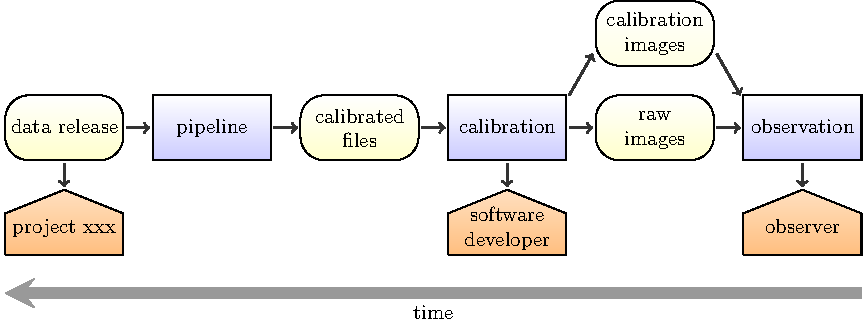
\includegraphics[width=1\textwidth]{workflow-backwards.pdf}
\caption[Example graph of provenance discovery]{An example graph of provenance discovery. Starting with a released dataset (left), the involved activities (blue boxes), 
progenitor entities (yellow rounded boxes) and responsible agents (orange pentagons) are 
discovered.}
\label{fig:example-workflow}
\end{figure}


The currently discussed Provenance Data Model is sufficiently abstract that its core pattern could be applied to any kind of process using either observation or simulation data.
It could also be used to describe the workflow for observation proposals or the publication of scientific articles based on (astronomical) data. However, here we focus on astronomical data. The links between the Provenance Data Model and other IVOA data models 
will be discussed in Section~\ref{sec:dmlinks}. We note here that the provenance of simulated data is already covered by the Simulation Data Model
\citep[SimDM,][]{std:SimDM}. Therefore we also give a mapping between SimDM and the Provenance Data Model in Section~\ref{sec:dmlinks}.


%including extraction of data from 
%databases or even the flow of scientific proposals from application to 
%acceptance, including scheduling of the observations proposed therein.
%Provenance information could also be used to check internal processes,
%e.g., whether a proposal was approved by a person from a certain committee,
%or whether the time span between application and acceptance or rejection
%does not extend a certain period, etc... 


\subsection{Goal of the provenance model}\label{sec:goals}

The goal of this Provenance Data Model is to describe how provenance information
can be modeled, stored and exchanged. Its scope
is mainly modeling of the flow of data, of the relations between data,
and of processing steps. 

Characteristics of observation activities such as ambient conditions and instrument characteristics can be associated to provenance information.  during the execution of processing activities (computer structure, nodes, operating system used\dots) can also be connected to provenance information. However, they will not be modeled here explicitly. This additional information can be included in the form of data or entities linked to those activities, or as attributes of activities (see also Section ~\ref{sec:parameters} for parameters of activities).

In general, the model shall capture information in a machine-readable way that would enable a scientist who has no prior knowledge about a dataset to get more background information. 
This will help the scientist to decide if the dataset 
is adequate for her research goal, assess its quality and get enough information
to be able to trace back its history as far as required or possible. 

Provenance information may be recorded in minute detail or by using coarser
elements, depending on the intended usage and the desired level of detail
for a specific project that records provenance. 
This granularity depends on the needs of the project and the intended usage when implementing a system to track provenance information.
% NOTE: maybe we need to define minimal requirements of what needs to be included as provenance information?

The following list is a collection of tasks which the Provenance Data Model should help to solve. They are flagged with [S] for problems which are more interesting for the end user of datasets (usually a scientist) and with [P] for tasks that are probably more important for data producers and publishers.
More specific use cases in the astronomy domain for different types of datasets and workflows along with example implementations are given in Section \ref{sec:usecases-implementations}.


\paragraphlb{A: Tracking the production history [S]}
        Find out which steps were taken to produce a dataset and list the methods/tools/software that was involved. 
        Track the history back to the raw data files/raw images, show the workflow (backwards search) or return a list of progenitor datasets.

        \noindent Examples: 
        \begin{itemize}
            \item Is an image from catalogue xxx already calibrated?
What about dark field subtraction? Were foreground stars removed? Which technique
was used?  
            \item Is the background noise of atmospheric muons still present in my neutrino data sample?  
        \end{itemize}

        We do not go as far as to consider easy reproducibility as a use case -- this would be too ambitious. But at least the 
        major steps undertaken to create a piece of data should be recoverable.


\paragraphlb{B: Attribution and contact information [S]}
        Find the people involved in the production of a dataset,
        the people/organizations/institutes that need to be cited or can be asked for more information.

        \noindent Examples: 
        \begin{itemize}
            \item I want to use an image for my own work -- who was involved in
creating it? Who do I need to cite or who can I contact to get this information? Is a license attached to the data? 
            \item I have a question about column xxx in a data
table. Who can I ask about that?  
            \item Who should be cited or acknowledged if I use this data in my work?
        \end{itemize}


\paragraphlb{C: Locate error sources [S, P]}
        Find the location of possible error sources in the generation of a dataset.

        \noindent Examples:
        \begin{itemize}
            \item I found something strange in an image. Where does
the image come from? Which instrument was used, with which characteristics
etc.? Was there anything strange noted when the image was taken?  
            \item Which pipeline version was used -- the old one
with a known bug for treating bright objects or a newer version?  
            \item This light curve doesn't look quite right. How was
the photometry determined for each data point?  
        \end{itemize}


\paragraphlb{D: Quality assessment [P]}
        Judge the quality of an observation, production step or dataset.
        
        \noindent Examples:
        \begin{itemize}
            \item Since wrong calibration images may increase the
number of artifacts on an image rather than removing them, knowledge about
the calibration image set will help to assess the quality of the calibrated
image.  
        \end{itemize}
      

\paragraphlb{E: Search in structured provenance metadata [P, S]}
        This would allow one to also do a ``forward search'', i.e. locate derived datasets or outputs, e.g. finding all images produced by a certain processing step or derived from data which were taken by a given facility.
        
        \noindent Examples:
        \begin{itemize}
            \item Give me more images that were produced using the same pipeline.  
            \item Give me an overview on all images reduced with the same calibration dataset.  
            \item Are there any more images attributed to this observer?  
            \item Which images of the Crab Nebula are of good quality and were produced within the last 10 years by someone not from ESO or NASA?
            \item Find all datasets generated using this given algorithm for this given step of the data processing
          % add another specific use case for tracking scientific productivity?
        \end{itemize}

        This task is probably the most challenging. It also includes tracking the history of data items as in A, but we still have listed this task separately, since we may decide that we can't keep this one, but we definitely want A.

\subsection{Minimum requirements for provenance}\label{sec:requirements}

We derived from our goals and use cases the following minimum requirements for the Provenance Data Model:

\begin{itemize}


% == other models / serialisation

\item Provenance information must be stored in a standard model, with standard serialization formats.

\item Provenance information must be machine readable.

\item Provenance data model classes and attributes should be linked to other IVOA concepts when relevant (DatasetDM, ObsCoreDM, SimDM, VOTable, UCDs, \ldots).

\item Provenance information should be serializable into the W3C provenance standard formats (PROV-N, PROV-XML, PROV-JSON) with minimum information loss.


% == links between entity/activity

\item Provenance metadata must contain information to find immediate progenitor(s) (if existing) for a given entity, i.e. a dataset.
%All produced entities must contain information to find its immediate progenitor(s).


\item An entity must be linked to the activity that generated it (if the activity is recorded).
%Provenance metadata must contain information to find the activity that generated a given entity.
%* All produced entities must contain information to find the activity that generated it

\item Activities must be linked to input entities (if applicable).

\item Activities may point to output entities.

\item Provenance information should make it possible to derive the chronological sequence of activities.
%The order of the activities should be available.

%\item Provenance information should contain the list of activities and progenitor entities.
% too vague .... must be an ordered list ... One step should also be allowed.
\end{itemize}

% ==== Comment: 
%These links can be used to trace back the sequence of processing steps (activities) and possibly the interim results.


% == additional information

\begin{itemize}

% Released entities must have a unique, persistent identifier (DOI, obs_publisher_did, ...), at least in their domain.
\item Entities, Activities and Agents must be uniquely identifiable within a domain and should have persistent identifiers.
% Provenance information can only be given for uniquely identifiable entities, at least inside their domain.
% comment: (DOI, obs_publisher_did, ...)
% Thus entities have to have a unique, persistent identifier.
% (to avoid ambiguities).

\item Released entities should have a main contact.

\item All activities and entities should have contact information and contain a (short) description or link to a description.
% could also be the documentation.

\end{itemize}


% Should this go into the requirements or the model?
%\item Activities should be defined by following keywords (attributes):
%    \begin{itemize}
%    \item unique ID
%    \item status (COMPLETED/ERROR/...)
%
%... (see working draft and data model)
%* Entities should be defined by... (see working draft and data model)


\subsection{Role within the VO architecture}

The IVOA Provenance Data Model is structuring and adding metadata to trace the original process followed during the data production to provide astronomical data. Even if it borrows the main general concepts defined from the data management science, it binds to the specific context of astronomical metadata description and re-uses or interacts with existing IVOA models.
It takes benefits from existing IVOA notations and standards like UCD, VOUnits, VO protocols and service design and is planned for a full integration into the VO landscape.

\begin{figure}
\centering
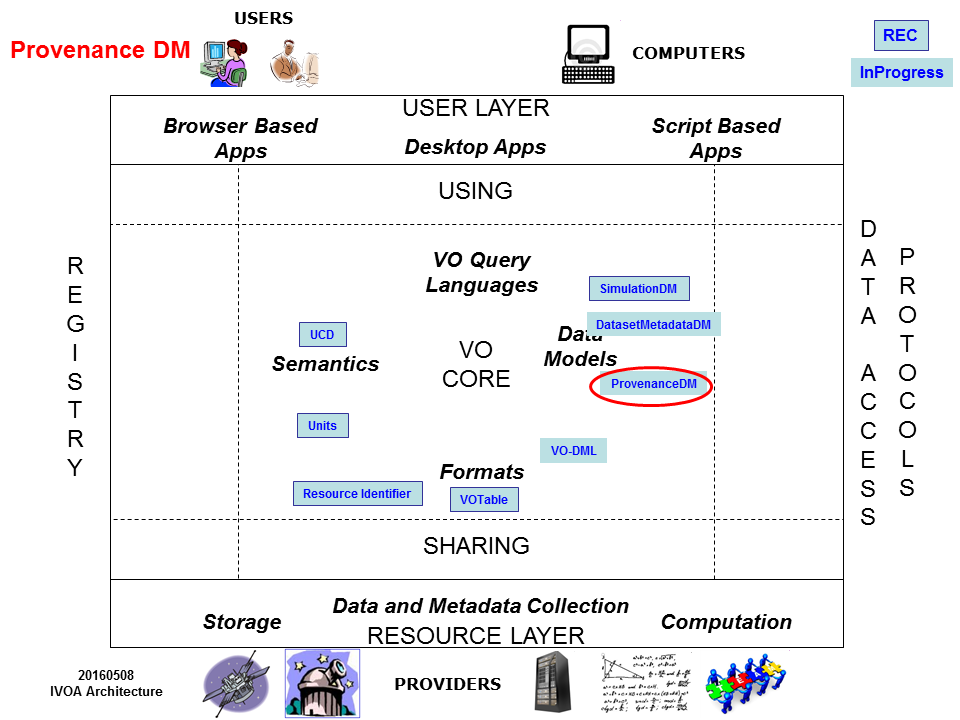
\includegraphics[width=0.9\textwidth]{VOArchitecture-Prov2016.png}
\caption{Architecture diagram for the Provenance Data Model. It is based on existing concepts defined in existing IVOA data models, and existing formats and semantics and fully integrated in the IVOA framework}
\label{fig:archdiag}
\end{figure}

Fig.~\ref{fig:archdiag} shows the dependencies of this document with respect to other existing standards.
%IVOA architecture \citep{note:VOARCH}.

\subsection{Previous efforts}
The provenance concept was early introduced by the IVOA within the scope of the Observation Data Model (ref1 : IVOA note 2005) as a class describing where the data are coming from. A full observation data model dedicated to the specific spectral data was then designed (Ref2 : spectral data model) as well as a fully generic characterisation data model of the measureemnt axes of the data (ref3: characterisation data model) while the progress on the provenance data model were slowing down.

IVOA DM WG first gathered various use cases coming from different communities of observational  astronomy (optical,  radio, Xray, interferometry). Common motivations for a provenance tracing of the history included : quality assesment, discovery of dataset progenitors and access to metadata necessary for reprocessing. Provenance datamodel was then designed as the combination of Data processing, Observing Configuration and Observation ambiant conditions datamodel classes. 
The Processing class was embedding a sequence of processing stages which were hooking specific ad hoc details and links to input and output datasets, as well as processing step description. 
Despite the attempts of UML description of the model and writing of xml serialization examples the IVOA effort failed to provide a workable solution:  the scope was probably too ambitious and the technical background too instable. A compilation of these early developments can be found on the IVOA site (ref4). From 2013 onwards IVOA concentrated on use cases related to processing description and decided to design the model  by extending the basic W3C provenance basic structure,as described in the current specification. 

Outside of the astronomical community, the Provenance Challenge series (2006 -- 2010), a community effort to achieve inter-operability between different representations of provenance in scientific workflows, resulted in the Open Provenance Model (\cite{moreau2010}). 
Later, the W3C Provenance Working Group was founded and released the W3C Provenance Data Model as Recommendation in 2013 (\cite{std:W3CProvDM}). 
OPM was designed to be applicable to anything, scientific data as well as cars or immaterial things like decisions. With the W3C model, this becomes more focused on the web.  Nevertheless, the core concepts are still in principle the same in both models and very general, so they can be applied to astronomical datasets and workflows as well. 
The W3C model was taken up by a larger number of applications and tools than OPM, we are therefore basing our modeling efforts on the W3C Provenance data model, making it less abstract and more specific, or extending it where necessary. 


The W3C model even already specifies PROV-DM Extensibility points (section 6 in \cite{std:W3CProvDM}) for extending the core model. This allows one to specify additional roles and types to each entity, agent or relation using the attributes \texttt{prov:type} and \texttt{prov:role}.
By specifying the allowed values for the IVOA model, we can adjust the model to our needs while still being compliant to W3C.



\section{The provenance data model}
In this section, we describe the currently discussed Provenance Data Model. We 
start with an UML class diagram, explain the core elements and then give 
in the following sections more details for each class and relation.

\subsection{Overview: UML class diagram and introduction to core classes}
 %We give in this section an overview on the main classes. More details about 
%each class and their relations will be explained in the following sections.
%Its core elements are colored in blue. These core elements can also be found in the W3C Provenance Data
%Model. The pattern defined by these classes is very general and can be reused everywhere where provenance is needed. 

\begin{figure}[h]
\centering
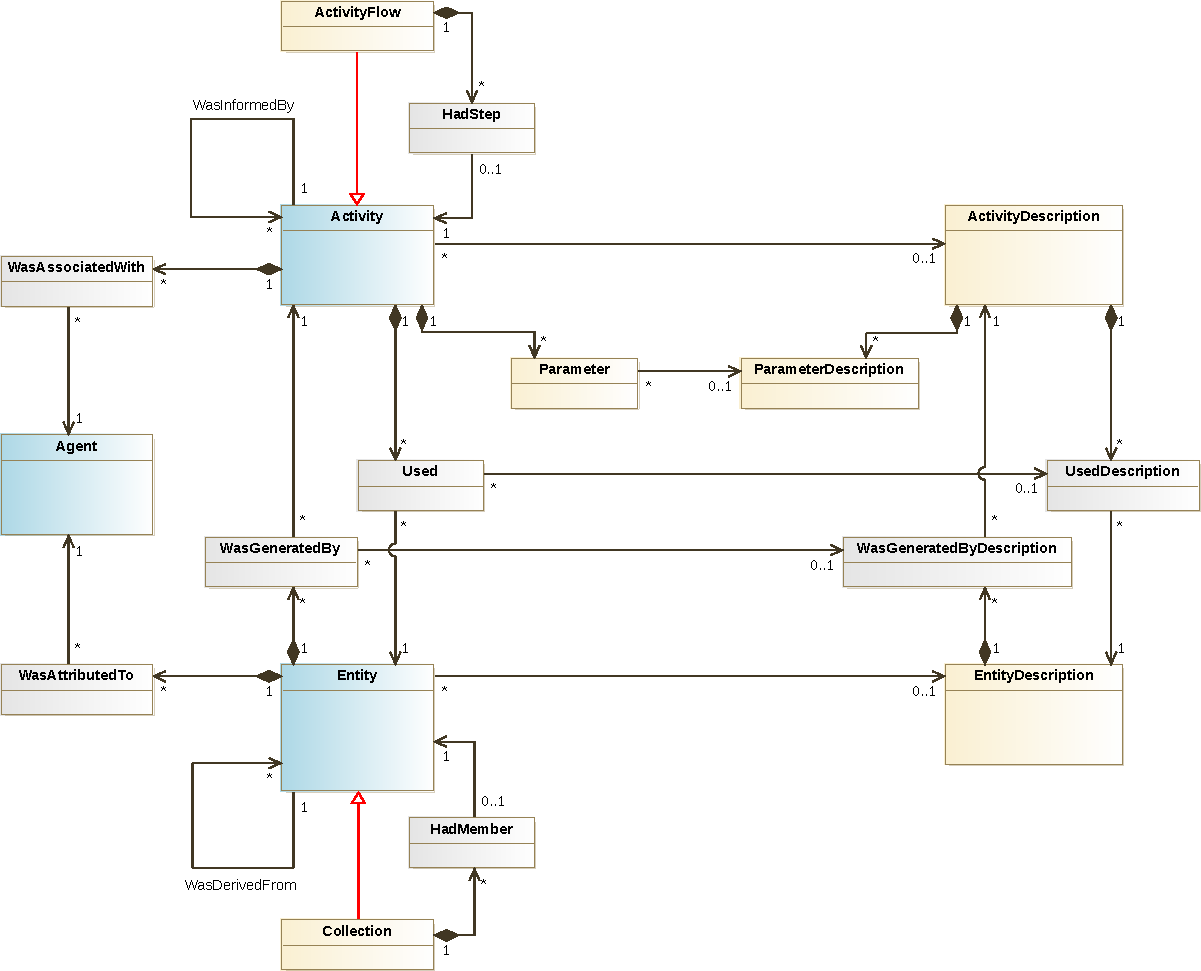
\includegraphics[width=1.0\textwidth]{../datamodel-diagrams/classes-overview.pdf}
\caption{Overview of the classes for the Provenance Data Model in a class diagram. The blue classes are core elements.
%Objects in the blue box also appear in the W3C Provenance Data Model. 
Green classes are links to the IVOA Dataset Metadata Model.}
\label{fig:classdiagram}
\end{figure}


%\label{sec:core}
% Some examples for different use cases are given in Section \ref{sec:usecases-implementations}.
% The elements of a provenance model can be expressed as a directed graph to capture the causal dependencies. 

Figure~\ref{fig:classdiagram} shows the UML diagram for an IVOA Provenance Data
Model.
The core elements of the Provenance Data Model are \class{Entity}, \class{Activity} and \class{Agent}. 
We chose for these elements the same names as were used in the Provenance Data 
Model of the World Wide Web Consortium (W3C, \citealt{std:W3CProvDM}), which defines 
a very abstract pattern that can be reused here. Here are the core classes with 
a short description and some examples:

\begin{itemize}
\item \class{Entity:} a thing at a certain state\\
    examples: data products like images, catalogs, parameter files, calibration data, instrument characteristics

\item \class{Activity:} an action/process or a series of actions, occurs over a period of time, performed on or caused by entities, usually results in new entities\\
    examples: data acquisition like observation, simulation; regridding, fusion, calibration steps, reconstruction

\item \class{Agent:} executes/controls an activity, is responsible for an activity or an entity\\
    examples: telescope astronomer, pipeline operator, principal investigator, software engineer, project helpdesk

\end{itemize}

\noindent



\begin{figure}[h]
\centering
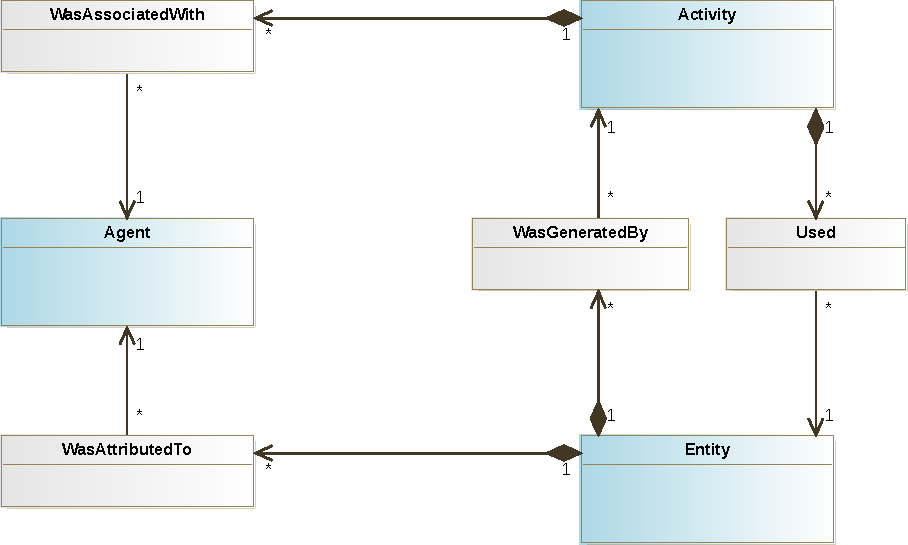
\includegraphics[scale=0.8]{../datamodel-diagrams/classes-core-w3c}
\caption{The main core classes and relations of the Provenance Data Model, which also occur in the W3C model.}
\label{fig:coreclasses}
\end{figure}

These core classes along with their relations to each other are provided in Figure~\ref{fig:coreclasses}.
We use the following relation classes to specify the mapping between the three core 
classes. The names were again chosen to match the W3C model names:
\begin{itemize}
\item \class{WasGeneratedBy:} a new entity is generated by an activity\\
        (entity ``image m31.fits'' wasGeneratedBy activity ``observation'')
\item \class{Used:} an entity is used by an activity\\
        (activity ``calibration'' used entities ``calibration data'', ``raw images'')
\item \class{WasAssociatedWith:} agents have responsibility for an activity\\
        (agent ``observer Max Smith'' wasAssociatedWith activity ``observation'')
\item \class{WasAttributedTo:} an entity can be attributed to an agent\\
		(entity ``image m31.fits'' wasAttributedTo ``M31 observation campaign'')
\end{itemize}


In the domain of astronomy, certain processes and steps are repeated again and 
again with different parameters. We therefore separate the descriptions of activities
from the actual processes and introduce an additional \class{ActivityDescription} class (see Figure~\ref{fig:classdiagram}).
Likewise, we also apply the same pattern for \class{Entity} and add an \class{EntityDescription}
class.
Defining such descriptions allows them to be reused, which is very useful 
when performing a series of tasks of the same type, as is typically done in 
astronomy. 

A similar normalization of descriptions of the actual processes and datasets 
can also be found in the IVOA Simulation Data Model \citep[SimDM, ][]{std:SimDM}), 
which describes simulation metadata. The SimDM classes \class{Experiment} and \class{Protocol} 
correspond to the Provenance terms \class{Activity} and \class{ActivityDescription}.

%The W3C-model has the advantage of being already an approved standard, and it 
%contains all the necessary main features needed for a Provenance model for 
%Astronomy. However, it is very general, and by adding reusable prototypes, 
%templates or descriptions for activities and entities,  the model may fit better 
%to the astronomy domain.

This separation into two classes may not be needed for each and every project,
and everyone is free to choose which classes make sense for his/her use case.
When serializing provenance, one could integrate the description side into the 
other classes, thus producing a W3C compliant provenance description. More details about 
all these classes and relations are given in the following section.


%It still remains to be seen if this separation into two classes is necessary, 
%useful or just nice to have. Currently, we include the descriptions in our model, 
%for normalization purposes. 

%But when serialising the provenance one could 
%integrate the description side into the other classes, thus producing W3C 
%compliant provenance.


\subsection{Model description}
\subsubsection{Entity and EntityDescription}
Entities in astronomy are usually astronomical or astrophysical datasets in the 
form of images, tables, numbers, etc. But they can also be observation or 
simulation log files or, in a wider sense, also observation proposals, scientific 
articles, or manuals and other documents. An entity is not restricted to being
a file. 
It can even be just a number in a table, depending on how fine-grained the 
provenance shall be described.

\begin{figure}[h]
\centering
\includegraphics[scale=0.7]{../datamodel-diagrams/entity-details}
\caption{The relation between Entity, Dataset and Collection (see Section~\ref{sec:collection}). 
The Dataset class as well as the classes with green boxes belong to
the IVOA Dataset Metadata Model. Some attributes of Dataset actually link to Entity-attributes, 
see Section~\ref{sec:dmlinks} for more details.}
\label{fig:entity-details}
\end{figure}

Entities in the VO are often called ``dataset'', which could mean a single 
table, an image or a collection of them. The Dataset Metadata Model 
\citep{std:DatasetDM} specifies an ``IVOA Dataset'' as ``a file or files which 
are considered to be a single deliverable''. 
Most parts of the \class{Dataset} class can be mapped
directly to the \class{Entity} class, as indicated in Figure \ref{fig:entity-details}.
If no \class{EntityDescription} is used, then most parts of the \class{Dataset} class can be mapped
directly to the \class{Entity} class or its description class \class{EntityDescription},
as indicated in Figure \ref{fig:entity-details}.
The detailed mapping of classes and attributes from the Dataset Metadata Model 
to \class{Entity}/\class{EntityDescription} are given in Section \ref{sec:dmlinks}. 


\begin{table}[h]

\small
\tymax	0.5\textwidth

\textbf{\normalsize Entity}\vspace{0.25em}\\
\begin{tabulary}{1.0\textwidth}{@{}lp{3.5cm}p{2cm}L@{}}
\toprule
\head{Attribute} & \head{W3C ProvDM} & \head{Data type} & \head{Description}\\
\midrule
\textbf{id} & prov:id & (qualified) string & a unique id for this entity (unique in its realm)\\
label       & prov:label & string & a label (to be displayed by clients)\\
type        & prov:type  & string & a provenance type, i.e. one of: prov:collection, prov:bundle, prov:plan, not needed for a simple entity\\
description\_link  & & foreign key/url & link to \class{EntityDescription}\\
annotation  & prov:description & string & text describing the entity in more detail\\
access      & -- & string & access rights for the data, values: public, restricted or internal; can be linked to Curation.Rights from ObsCore/DatasetDM\\
\bottomrule
\end{tabulary}
\caption{Attributes of entities. Mandatory attributes are marked in bold.
}\label{tab:entity-attributes}
\end{table}

For entities, we suggest the attributes given in Table 
\ref{tab:entity-attributes}. If the attribute also exists in the W3C 
Provenance Data Model, we list its name in the second column.
We discussed further attributes like \emph{size} and \emph{format}, but we decided to treat an
entity of the same content but different format (and thus size) as the same entity,
unless they do not have the same provenance (e.g. when the ``transformation'' activity
for converting one format into another is included in the provenance description).

%\TODO{format and size may not be needed, if entities with the same content but different format and size are considered as the same entity.}

The difference between entities that are used as input data or output data 
becomes clear by specifying the relations between the data and activities producing or using these data.
More details on this will follow in Section \ref{sec:entity-activity-relations}.

\paragraph{EntityDescription.}
As already mentioned before, the types of entities or datasets in astronomy 
can be predefined using a description
class \class{EntityDescription}.
This class stores entity-related 
attributes, describing the content of the data, which can mainly be derived from 
the Dataset Metadata Model, the general model for observational data.
The description attributes are summarized in Table 
\ref{tab:entitydescription-attributes}.

The \class{EntityDescription} does NOT contain any information about the usage 
of the data, it tells nothing about them being used as input or output. This is 
defined only by the relations (and the relation descriptions) between activities
and entities (see Section \ref{sec:entity-activity-relations}).


\begin{table}[h]
\small
\tymax	0.5\textwidth
\textbf{\normalsize EntityDescription}\vspace{0.25em}\\
\begin{tabulary}{\textwidth}{@{}p{2.75cm}p{0cm}p{2cm}L@{}}
\toprule
\head{Attribute} & \head{} & \head{Data type} & \head{Description}\\
\midrule
\textbf{id} & & (qualified) string & a unique identifier for this description\\
label       & & string & a name or label for the entity description\\
annotation  & & string & a decription for this kind of entity\\
docu\_link    & & url & link to more documentation\\
dataproduct\_ type  & & string       & from ObsCore data model \citep{std:ObsCore}, if applicable; describes, what kind of product it is (e.g. image, table)\\
dataproduct\_ subtype & & string       & from ObsCore data model, more specific subtype\\
level       & & enum integer & the level of processing or calibration; for ObsCore's calib\_level it is an integer between 0 and 3\\
\bottomrule
\end{tabulary}
\caption{Attributes of \class{EntityDescription}. For simple use cases, 
the description classes may be ignored and its attributes may be used for 
\class{Entity} instead. 
%The utypes may vary depending on the data model, e.g. for simulation data they 
%would point to utypes of SimDM.
}\label{tab:entitydescription-attributes}
\end{table}

\paragraph{WasDerivedFrom.}
In Figure~\ref{fig:entity-details} there is one more relation that we have not mentioned yet: 
the \class{WasDerivedFrom}-relation which links two entities together, borrowed from the W3C model. 
Is is used to express that 
one entity was derived from another, i.e. it can be used to find one (or more) progenitor(s) 
of a dataset, without having to mention the activities in between. It can therefore serve as 
a shortcut. The information this link provides is somewhat redundant, since progenitors for entities
can be found through the links to activity and the corresponding descriptions.
Nevertheless, we include \class{WasDerivedFrom} for those cases where an explicit 
link between an entity and its progenitor is useful (e.g. for speeding up searches for 
progenitors or if the activity in between is not important).



\subsubsection{Collection}\label{sec:collection}
Collections are entities that are grouped together and can be treated as one single entity. 
From the provenance point of view, they have to have the \emph{same origin}, i.e., they were 
produced by the same activity (which could also be the activity of collecting
data for a publication or similar). The term ``collection'' is 
also used in the Dataset Metadata Model for grouping datasets.
% (but with a slightly different meaning). 
As an example, a collection 
with the name `RAVE survey' could consist of a number of database tables and spectra files.

%\TODO{Do we allow empty collections? Or should collections always contain at least 1 member? (otherwise they are just prov:entities?)}

The Entity-Collection relation can be modeled using the \emph{Composite} design pattern: 
Collection is a subclass of Entity, but also an aggregation of 1 to many entities, 
which could be collections themselves. 
In order to be compliant to VODML, we model the membership-relation explicitely 
by including a \class{HadMember} class in our model, which is connected to the
\emph{Collection} class via a composition. It may contain an additional role attribute.

Collections are also known in the W3C model, in the same sense as used here.
The relation between entity and collection is also called ``HadMember'' in the W3C model.

An additional class \class{CollectionDescription} is only 
needed if it has different attributes than 
the \class{EntityDescription}. This class should therefore only be introduced if a use case requires it.

\paragraph{Advantages of collections:} Collections can be used to collect entities with the same provenance information together, 
    in order to hide complexity where necessary. They can be used for defining 
    different levels of detail (granularity).


%\TODO{Find a really strong use case for Collections to convince everyone that they are useful/needed.}



\subsubsection{Activity and ActivityDescription}

\begin{figure}[h]
\centering
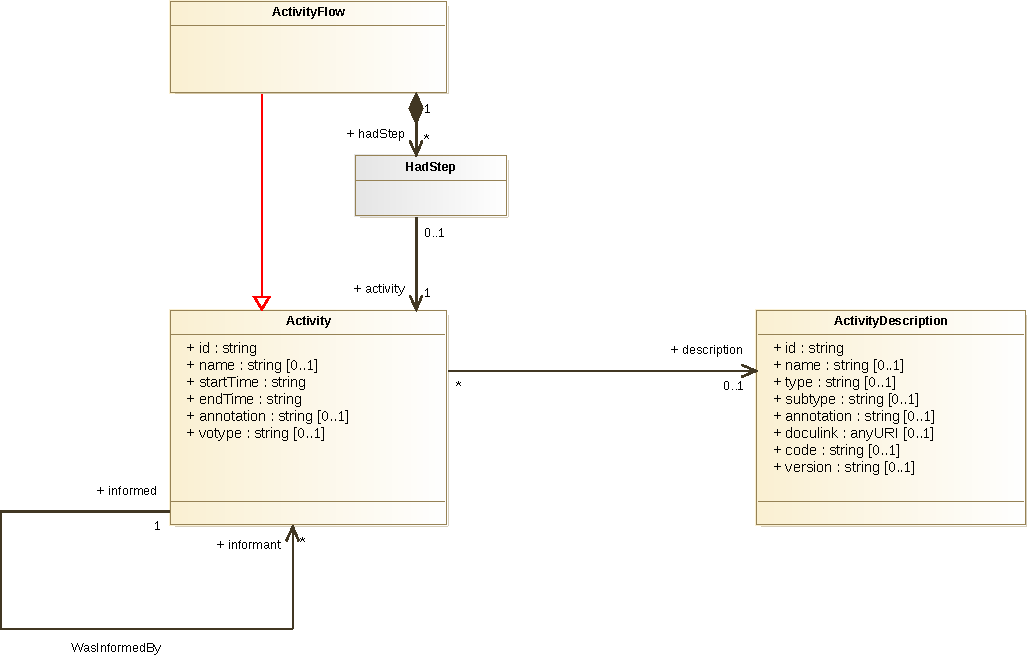
\includegraphics[scale=0.5]{../datamodel-diagrams/activity-details.pdf}
\caption{Details for Activity, ActivityDescription and ActivityFlow (see Section~\ref{sec:activityflow}). 
}
\label{fig:activity-details}
\end{figure}



\begin{table}[h]

\small
\tymax  0.5\textwidth

\textbf{\normalsize Activity}\vspace{0.25em}\\
\begin{tabulary}{1.0\textwidth}{@{}lp{2.5cm}p{2cm}L@{}}
\toprule
\head{Attribute} & \head{W3C ProvDM} & \head{Data type} & \head{Description}\\
\midrule
\textbf{id} & prov:id  & (qualified) string & a unique id for this activity (unique in its realm)\\
label        & prov:label  & string & a label (to be displayed by clients)\\
\textbf{startTime} & prov:startTime & datetime & start of an activity\\
\textbf{endTime} & prov:endTime  & datetime & end of an activity\\
annotation        & prov:description & string & additional explanations for the specific activity instance\\
description\_link  &  & foreign key/url & link to \class{ActivityDescription}\\
\bottomrule
\end{tabulary}
\caption{Attributes of \class{Activity}, their data types and equivalents in the W3C Provenance 
Data Model, if existing. Attributes in bold are \textbf{mandatory}.}
\end{table}


\begin{table}[ht]
\small
\tymax  0.5\textwidth
\textbf{\normalsize ActivityDescription}\vspace{0.25em}\\
\begin{tabulary}{1.0\textwidth}{@{}p{0cm}p{2.5cm}lL@{}}
\toprule
\head{Attribute} & \head{} & \head{Data type} & \head{Description}\\
\midrule
\textbf{id}  & & string & a unique id for this activity description (unique in its realm)\\
label        & & string & a label (to be displayed by clients)\\
type         & & string & type of the activity, from a vocabulary or list, e.g. data acquisition (observation or simulation), reduction, calibration, publication\\
subtype      & & string & more specific subtype of the activity\\
annotation  & & string & additional free text description for the activity\\
%code         & & string & the code used for this process\\
%version      & & string & a version number for the code\\
docu\_link     & & url    & link to further documentation on this process, e.g. a 
paper, the source code in a version control system etc.\\
\bottomrule
\end{tabulary}
\caption{Attributes of \class{ActivityDescription}.}
\end{table}


Activities in astronomy include all steps from obtaining data to the reduction of 
images and production of new datasets, like image calibration, bias subtraction, image stacking; 
light curve generation from a number of observations, radial velocity 
determination from spectra, post-processing steps of simulations etc.

\paragraph{ActivityDescription.}
The method underlying an activity can be specified by a corresponding 
\class{ActivityDescription} class (previously named \class{Method}, corresponds 
to the \class{Protocol} class in SimDM). This could be, 
for instance, the name of the code used to perform an activity or a more general 
description of the underlying algorithm or process. An activity is then a 
concrete case (instance) of using such a method, with a startTime and endTime, 
and it refers to a corresponding description for further information.

There MUST be exactly zero or one \class{ActivityDescription} per \class{Activity}. If steps from a 
pipeline shall be grouped together, one needs to create a proper 
\class{ActivityDescription} for describing all the steps at once. This method can then 
be refered to by the pipeline-activity. 

When serializing the data model, the attributes
of the description class may be assigned to the activity in order to produce 
a W3C compliant serialization (same as with Entity/EntityDescription).


\paragraph{WasInformedBy.}
The individual steps of a pipeline can be chained
together directly, without mentioning the intermediate datasets, using the \class{WasInformedBy}-relation.
This relation can be used as a short-cut, if the exchanged datasets are deemed to be not important
enough to be recorded. For grouping activities, also see the 
next section \ref{sec:activityflow}.


\subsubsection{ActivityFlow}\label{sec:activityflow}
For facilitating grouping of activities (and their related entities etc.)
we introduce the class \class{ActivityFlow}.
It can be used for hiding a part of the workflow or provenance 
description, if different levels of granularity are needed. Figure \ref{fig:provgraph-activityflow}
illustrates an example provenance graph in a detailed level (left side) 
and using the ActivityFlow (right side).


\begin{figure}[h]
\centering
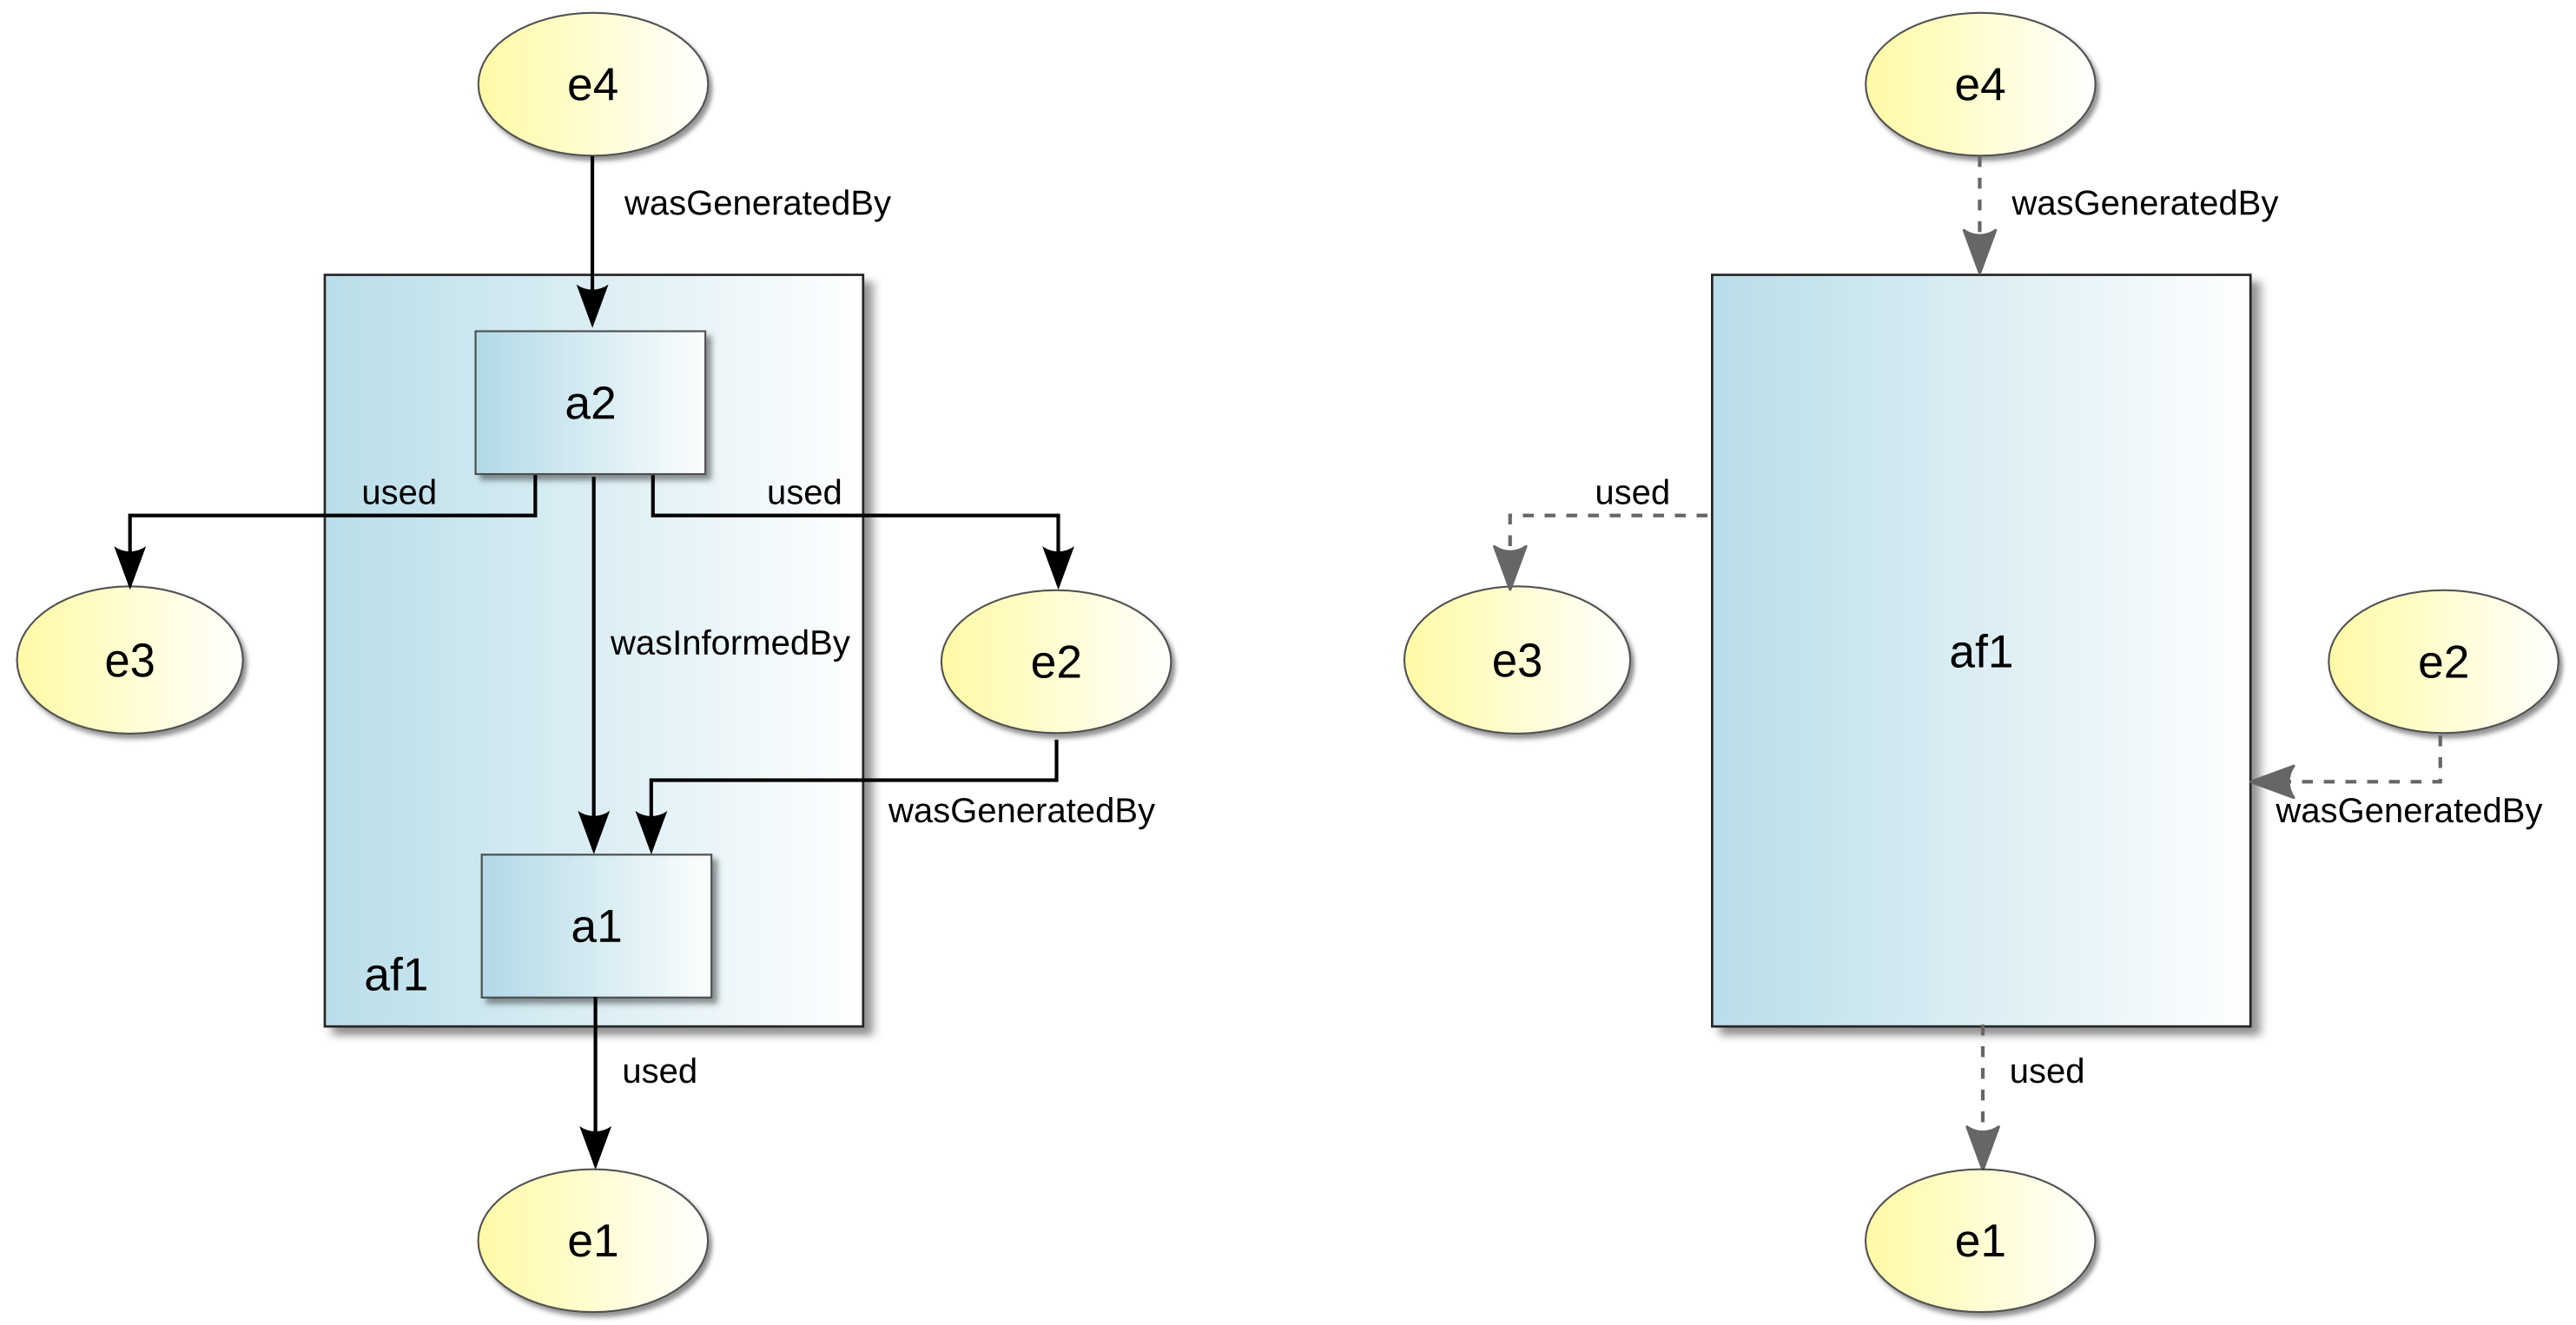
\includegraphics[width=1\textwidth]{../datamodel-diagrams/provgraph-activityflow}
\caption{An example provenance graph. The detailed version is shown on the left side. It also shows
the shortcut \class{WasInformedBy} to connect two activities, which could be used if the entity e2 
would not be needed anywhere else. 
An ActivityFlow can be used to ``hide'' a part of the provenance graph as is shown on the right side.
Activities are marked by blue rectangles, entities by yellow ellipses.}
\label{fig:provgraph-activityflow}
\end{figure}

%\TODO{BEWARE: Allowing this means that there can be 2 or more wasGeneratedBy-relations
%per entity!! This is currently NOT allowed in our model (multiplicity 0..1)! Or shall we 
%allow the encapsulating parts of a provenance graph 
%only in the view, i.e. on the implementation side?}


%In the W3C provenance model, the entity type \class{Plan} is used for workflows and 
%provenance descriptions are called \class{Bundle}. However, we do not reuse these 
%terms here, since we want to use the class \class{ActivityFlow} as a kind of \class{Activity}
%with all the relations and properties that belong to an \class{Activity}. 


We explored the different ways to describe a set of activities in the W3C 
provenance model. This model uses \class{Bundle}, i.e. an entity with type ``Bundle'', 
for wrapping a provenance description. Each part of a provenance description can be 
put into a bundle, and the bundle can then be reused in other provenance descriptions. 
W3C's \class{Plan} is an entity with type ``Plan'' and is used for describing a 
set of actions or steps. Both, \class{Bundle} and \class{Plan}, are entities and 
have the attributes and relations of this class (and thus one can define provenance of bundles and plans as well).

But we would like to consider a set of activities as being an \class{Activity} itself, 
with all the relations and properties that an activity also has. Therefore we do not reuse
W3C's classes for describing workflows and plans, but added 
the class \class{ActivityFlow} as an activity composed of activities. The composition is represented by 
the ``hadStep'' relation, as is shown in Figure~\ref{fig:activity-details}.

%while still making it obvious that this 
%group contains activities, we introduce the class \class{ActivityFlow}.
%This can be used for describing workflows or pipelines, or for 
%
%We also allow ActivityCollections to consist of a whole provenance graph of 
%activities and entities being linked together.



\subsubsection{Entity-Activity relations}\label{sec:entity-activity-relations}

For each data flow it should be possible to clearly identify entities and 
activities. 
%If the activities shall not be recorded explicitely, one could also 
%use the \emph{Derivation}-relation as suggested in the W3C Provenance Data Model
%to link derived entities to their originals.
Each entity is usually a result from an activity, expressed by a link from 
the entity to its generating activity using the \class{WasGeneratedBy} relation,
and can be used as input for (many) other activities, expressed by the \class{Used} relation.
Thus the information on whether data is used as input or was produced as output of 
some activity is given by the \emph{relation-types} between activities and entities.
%In fact, 
%it would be enough to provide this information just for the relations on the description side (right).
% -- Is this true?

We use two relations, \class{Used} and \class{WasGeneratedBy}, instead of just one
mapping class with a flag for input/output, because their descriptions and role-attributes
can be different. 
%in order to model the different 
%multiplicities explicitely: an entity always has only one (or none) 
%\class{WasGeneratedBy} relation, but may be \class{Used} many times as input for 
%different activities.
In previous versions of this model we only allowed one wasGeneratedBy-activity per 
entity. However, we introduced in Section~\ref{sec:activityflow} the additional \class{ActivityFlow} as 
a subclass to \class{Activity} for grouping activities together. Thus we need to 
weaken the constraint and allow more than one wasGeneratedBy-activity per entity. 

Each activity requires specific roles for each input or output entity, thus 
we store this information on the description side, in the role-attributes for 
the \class{UsedDescription} and \class{WasGeneratedByDescription} relation.
For example, an activity for darkframe-subtraction requires two input images. But it is 
very important to know which of the images is the raw image and 
which one fulfills the role of dark frame.

The role is in general NOT an attribute for \class{EntityDescription} or \class{Entity}, 
since the same entity (e.g. a specific fits file containing an image) may play 
different roles with different activities. If this is not the case, if the 
image can only play the same role everywhere, only then it is an intrinsic 
property of the entity and should be stored in the \class{EntityDescription}.

%Additionally, input (and also output) data can take different roles in an 
%activity. For example, one file could
%be a parameter file, another one is the raw image, and the third one is the 
%dark field that should be subtracted. Since these roles are very important, 
%it must be made explicit which data component needs to fulfill which role as 
%input in or output from an activity.
%Each activity requires specific roles for each input or output entity, thus 
%we store this information on the description side, in the role-attributes for 
%the \class{UsedDescription} and \class{WasGeneratedByDescription} relation.

%In W3C, this is partially solved by adding a derivation relation between the Entities (data). Here, we have a mapping-class between Activity and DataEntities as well as between ActivityDescription and DataDescription. The mapping-class at the description side, i.e. between the ActivityDescription and its DataEntityDescriptions, contains additionally a role for each relation, e.g. parameter, dark frame, raw image, etc.  If a dataset is used as input to an activity or if it results from it, will become clear with these roles.


Some example roles are given in Table \ref{tab:entity-roles}.
Note that these roles don't have to be unique, many datasets may play the same role for 
a process. For example, many image entities may be used as science-ready-images for an 
image stacking process.

\begin{table}[h]
\small
\begin{tabulary}{1.0\textwidth}{@{}L@{}}
\toprule
\head{Name} \\%& \head{Description}\\
\midrule
parameter \\%& \\
dark frame \\%& \\
calibration image \\%& \\
raw image \\%& \\
science-ready image \\%& \\
\bottomrule
\end{tabulary}
\caption{Example values for the entity roles as attributes in the 
\class{UsedDescription} and \class{WasGeneratedByDescription}.}
\label{tab:entity-roles}
\end{table}


In order to facilitate interoperability, the possible 
entity-roles could be defined and described for each activity by the IVOA community, in a 
vocabulary list or thesaurus.
% TODO!!


%\TODO{Roles can be used for checking (validation) if processes use the correct type of entities, 
%e.g. check if entity-type matches used-role!}

%Without the mapping tables, the relation between \class{Activity} 
%(\class{ActivityDescription}) and \class{Entity} (\class{EntityDescription})
%would be an aggregation relation, or in other words: an association with the 
%aggregation kind ``shared''. That would be required to ensure that all 
%entities linked to an activity (either as input or output) will survive if 
%the activity is destroyed, since they are almost always shared with other 
%activities. 
%
%By using the mapping tables we make the role of an entity in an activity more 
%explicit and thus can replace the aggregation by a composition relation to the 
%\class{Activity}/\class{ActivityDescription} and simple associations to the 
%individual data components and their descriptions. 


% The derivation relation together with entities is already enough to produce a 
% Data flow view, but in astronomy we are probably even more interested in the 
% Processes (as discussed in our first draft for requirements for provenance).

%\TODO{Add an example here! (From discussions in Heidelberg.)}



\subsubsection{Parameters}\label{sec:parameters}

The concept of activity configuration, generally a set of parameters that can be configured, is different to the concept of provenance information. However, it is tightly connected. We identify three different ways to link configuration information to an activity:
\begin{itemize}
\item Declare a parameter set (or each parameter) as an input entity that is used by the activity. \\
        This also allows tracking the provenance of the parameter further.
\item Define families of activities, each one with fixed attributes.\\
        I.e. use different subclasses for activities with different fixed attributes.
\item Add activity attributes in the form of key-value parameters.
\end{itemize}

To enable the latter solution, we add a \class{Parameter} class along with a \class{ParameterDescription} for describing additional properties of activities. In this solution, Parameters are directly connected to an Activity without complex Entity-Activity relations. Moreover, we can then describe each parameter in the same way as in FIELD and PARAM elements in VOTable \citep{std:VOTable}.


\begin{table}[h]
\small
\tymax  0.5\textwidth
\textbf{\normalsize Parameter}\vspace{0.25em}\\
\begin{tabulary}{1.0\textwidth}{@{}p{0cm}p{2.5cm}lL@{}}
\toprule
\head{Attribute} & \head{} & \head{Data type} & \head{Description}\\
\midrule
\textbf{id}      & & string & parameter unique identifier\\
description\_link   & & foreign key/url & link to \emph{ParameterDescription}\\
label            & & string & parameter name, if no link to ParameterDescription is given\\
\textbf{value}   & & (value dependent) & the value of the parameter\\
\bottomrule
\end{tabulary}
\caption{Attributes of \class{Parameter}. Attributes in bold are \textbf{mandatory}.}
\end{table}

\begin{table}[ht]
\small
\tymax  0.5\textwidth
\textbf{\normalsize ParameterDescription}\vspace{0.25em}\\
\begin{tabulary}{1.0\textwidth}{@{}p{0cm}p{2.5cm}lL@{}}
\toprule
\head{Attribute} & \head{} & \head{Data type} & \head{Description}\\
\midrule
\textbf{id}  & & string & parameter unique identifier\\
label         & & string & parameter name\\
annotation & & string & additional free text description for the parameter\\
datatype    & & string & datatype of the parameter \\
unit           & & string & physical unit of the parameter\\
ucd           & & string  & Unified Content Descriptor for the parameter, supplying a standardized classification of the physical quantity\\
utype        & & string  & UType of the parameter, meant to express the role of the parameter in the context of an external data model \\
\bottomrule
\end{tabulary}
\caption{Attributes of \class{ParameterDescription}.}
\end{table}

For example, observations generally require information on \emph{ambient conditions} as well as 
\emph{instrument characteristics}. This contextual data associated with an observation are not directly modelled in the ProvenanceDM. However, this information can be stored as different entities. Alternatively, one could list the instrument characteristics as a set of key-value parameters using the \class{Parameter} class, so that this information is structured and stored with the provenance information (and can thus be queried simultaneously). In the case of a processing activity that cleans an image with a sigma-clipping method, the input and output images would be an entity and the value of the number of sigma for sigma-clipping could be a parameter instead of an entity. We may also want to define a 3-sigma-clipping activity where this parameter is fixed to 3.


%For example for observations, the \emph{ambient conditions} as well as 
%\emph{instrument characteristics} need to be stored. But they can both be treated
%as additional entities as well. 
%Our model can then also take into account that a certain observation
%method requires special ambient conditions, already defined via the 
%ActivityDescription (e.g. radio observations rely on different ambient 
%conditions than observations
%of gamma rays), just following our data -- data description scheme.
%Ambient conditions are recorded for a certain time (startTime, endTime) and are
%usually only valid for a certain time interval. This time interval should be recorded
%with a \emph{validity}-attribute for such entities.
%
%In contrast to ambient conditions, instrument characteristics do (usually) not
%change from one observation to the other, so they are static, strictly related to
%the instrument. 
%All the characteristics could be described either as key-value pairs directly with the 
%observation (as attributes) or just as datasets, using the \class{Entity} class. 
%One would then 
%link the instrument characteristics as a type of input (or output?) dataset to a certain 
%observation activity. Thus we don't need a separate Instrument or Device class.

%\note{One should also keep in mind that some instrument related parameters can change within time,
%e.g. the CCD temperature. The instruments can also change within time because of aging.}



\subsubsection{Agent}\label{sec:w3c-agent}

An \class{Agent} describes someone who is responsible for a certain task or
entity, e.g. who pressed a button, 
ran a script, performed the observation or published a dataset.
The agent can be a single person, a group of persons (e.g. MUSE WISE Team), a 
project (RAVE) or an institute. 
This is also reflected in the IVOA Dataset Metadata Model, where \class{Party} 
represents an agent, and it has two subtypes: \class{Individual} and \class{Organization},
which are explained in more detail in Table \ref{tab:agent-types}.
Both types are also used for agent types in the W3C Provenance Data Model, though 
\class{Individual} is called \class{Person} there. 
We do not include the type \class{SoftwareAgent} from W3C, since it is not required for 
our use cases.

\begin{table}[h]
\small
\tymax  0.5\textwidth
\begin{center}
\begin{tabulary}{1.0\textwidth}{@{}lllL@{}}
\multicolumn{4}{c}{\textbf{AgentType}}\\
\toprule
\head{Class} & \head{W3C ProvDM} & \head{DatasetDM} &\head{Comment} \\
\midrule
Agent       & Agent  & Party & \\
Individual  & Person & Individual & a person, specified by name, email, address, 
      (though all these parts may change in time)\\
Organization & Organization & Organization & a publishing house, institute or scientific project\\
\bottomrule
\end{tabulary}
\caption{Types of agents}
\label{tab:agent-types}
\end{center}
\end{table}

A definition of organizations is given in the 
IVOA Recommendation on Resource Metadata \citep{std:ResourceMeta}, hereafter 
refered to as RM: ``An organisation is [a] specific type of resource that 
brings people together to pursue participation in VO applications.''
It also specifies further that scientific projects can be considered 
as organisations on a finer level:
``At a high level, an organisation could be a university, observatory, or government
agency. At a finer level, it could be a specific scientific project, space mission,
or individual researcher. A provider is an organisation that makes data and/or services
available to users over the network.''

For each agent a \emph{name} should be specified.
It would also increase the value of the given
information if the (current) affiliation of the agent (and a project leader/group
leader) were specified in order to maximize the chance of finding any contact 
person later on. 
The contact information is needed in case more information about a certain step in the past of a dataset is required,
but also in order
to know who was involved and to fulfill our ``Attribution'' requirement 
(Section~\ref{sec:requirements}), so that proper credits are given to the right 
people/projects.

\begin{figure}[h]
\centering
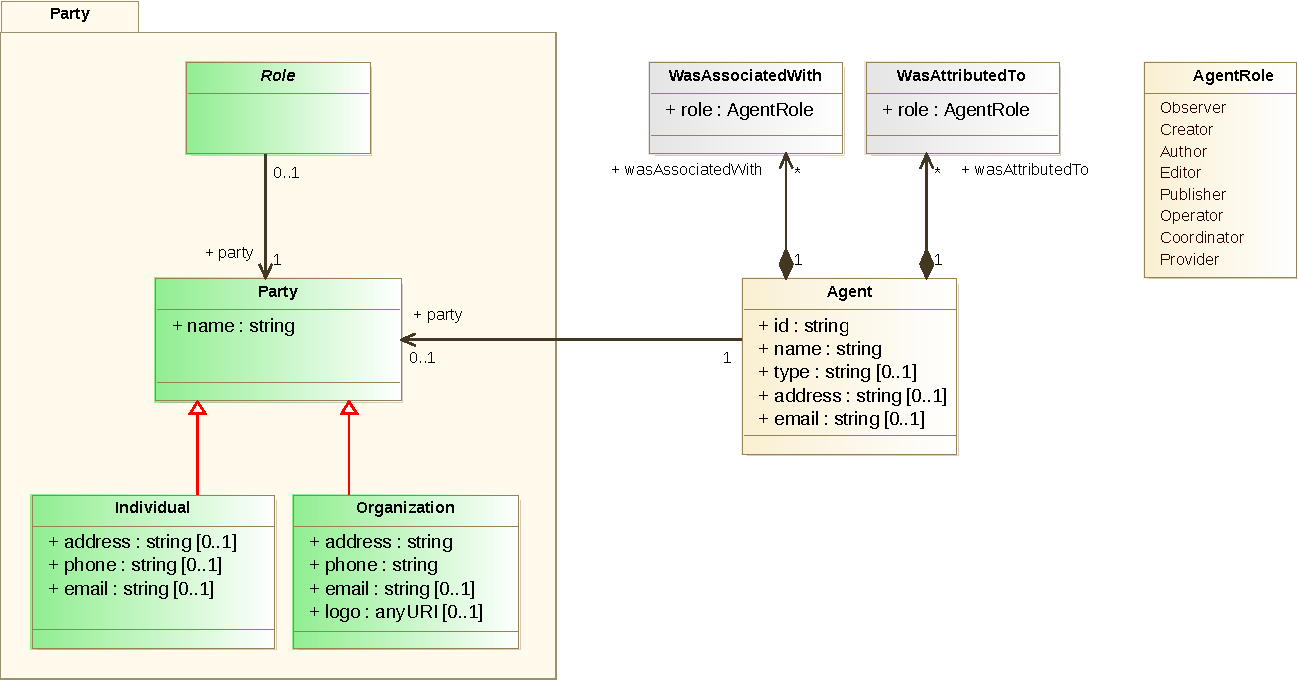
\includegraphics[scale=0.7]{../datamodel-diagrams/agent-relations.pdf}
\caption{The relations between the \class{Agent} class within the Provenance Data Model 
(grey and yellow classes) with classes from the Dataset Metadata Model (green).}
\label{fig:agent-relations}
\end{figure}


The relations between \class{Agent} and other classes from the Provenance Data Model and
the IVOA Dataset Metadata Model are detailed in Figure \ref{fig:agent-relations}.

It is desired to have at least one agent given for each activity (and entity), but it
is not enforced.
% , hence the multiplicity between \class{Entity}/\class{Activity} and the relations
%to the \class{Agent} starts with 0.
There also can be more than one agent for each activity/entity with different \emph{roles} 
and one agent can be responsible for more than one activity or entity. This 
many-to-many relationship is made explicit in our model by adding the two
following relation classes:

\begin{itemize}
\item wasAssociatedWith: relates an \emph{activity} to an agent
\item wasAttributedTo: relates an \emph{entity} to an agent
\end{itemize}

We adopted here the same naming scheme as was used in W3C ProvDM.
Note that the attributed-to-agent for a dataset may be different from the 
agent that is associated with the activity that created an entity. 
Someone who is performing a task is not necessarily given full attribution, 
especially if he acts on behalf of someone else (the project, university, ...).

In order to make it clearer what an agent is useful for, we suggest the
possible roles an agent can have (along with descriptions partially taken from RM)
in Table~\ref{tab:agent-roles}. 
For comparison, SimDM contains following roles 
for their \emph{Contact} class: 
owner, creator, publisher and contributor.


\begin{table}[h]
\small
\tymax	0.5\textwidth
\begin{center}
\begin{tabulary}{1.0\textwidth}{@{}lp{3cm}L@{}}
\multicolumn{3}{c}{\textbf{AgentRoles}}\\
\toprule
\head{prov:role} & \head{prov:type} & \head{Comment} \\
\midrule
author & prov:person & someone who wrote an article, software, proposal\\
contributor & prov:person & someone who contributed to something (but not enough to gain authorship)\\
editor & prov:person & editor of e.g. an article, before publishing\\
creator & prov:person & someone who created a dataset, creators of articles or software are rather called ``author''\\
curator & prov:person & someone who checked and corrected a dataset before publishing\\
publisher & prov:organization \mbox{(maybe also person?)}& organization (publishing house, institute) that published something\\
observer & prov:person & observer at the telescope\\
operator & prov:person & someone performing a given task (executor?)\\
coordinator/PI & prov:person & someone coordinating/leading a project\\
provider & prov:organization & ``an organization that makes data and/or services available to users over the network'' (definition from RM)\\
%(owner) & prov:person or prov:organization & Does anyone really own the data?\\
\bottomrule
\end{tabulary}
\caption{Examples for roles of agents and the typical type of that agent}
\label{tab:agent-roles}
\end{center}
\end{table}

%\TODO{\textbf{Mireille + Fran\c{c}ois}: Go through these roles, pick only the necessary ones, crosscheck with other data models.}

This list is \emph{not} complete. We consider providing a vocabulary list for this 
in a future version of this model, collected from (future) implementations of this model.

%\TODO{Do we have a specific use case for fixing the agent-roles? Is anyone 
%going to search for specific roles in the Provenance meta-data?
%Or shall we leave it open, which roles can be defined and just give examples here?}
% ... Yes, just give examples here. Should have a vocabulary list somewhere ...

\begin{table}[h]
\small
\tymax  0.5\textwidth
\begin{center}
\begin{tabulary}{1.0\textwidth}{@{}llp{2cm}L@{}}
\multicolumn{4}{c}{\textbf{Agent}}\\
\toprule
\head{Attribute} & \head{W3C ProvDM} & \head{Data type} & \head{Description}\\
\midrule
id & prov:id & (qualified) string & unique identifier for an agent\\
label & prov:name & string & a common name for this agent; e.g. first name and last name; project name, ...\\
type & prov:type & string & type of the agent: either Individual (Person) or Organization\\
\bottomrule
\end{tabulary}
\caption{Agent attributes}
\label{tab:agent-attributes}
\end{center}
\end{table}


%\subsubsection{Shortcuts: WasDerivedFrom and WasInformedBy}\label{sec:shortcuts}
%The classes \class{WasDerivedFrom} and \class{WasInformedBy} can be used as ``shortcuts'' and 
%are used in the same way as the corresponding W3C classes.

%\class{WasDerivedFrom} defines the relation that links two entities together, if one entity was derived
%from the other entity. In principle, one can find this information also by tracing the 
%history of an entity backwards to the generating activity and its input entities. 
%The descriptions for activity, entity and their relations should provide enough
%information to find the progenitor entity from which an entity was derived.
%Nevertheless, we include \class{WasDerivedFrom} for those cases where an explicite 
%link between an entity and its progenitor is useful (e.g. for speeding up searches for 
%progenitors or if the activity in between is not important).

%The class \class{WasInformedBy} links two activities together without defining the
%intermediate entities that may have been exchanged. This is useful for e.g. pipelines, 
%if the intermediate entities don't play a major role or only exist temporarily, so that
%their provenance information is not deemed to be important enough to be recorded.
%``WasInformedBy'' relation (also called ``Communication'' relation, borrowed from W3C's model) 


%\subsection{Implementation hints}



%\section{Applying provenance -- Interactions with other Data models}\label{sec:dmlinks}
\section{Links to other data models}\label{sec:dmlinks}
%In this section we discuss how the Provenance Data Model interacts with
%classes and attributes from other VO data models (especially DatasetDM).
%(e.g. DatasetDM, SpectralDM (share some same classes), SimDM) 
%and how provenance information can be stored.

The Provenance Data Model can be applied without making links to any other 
IVOA data model classes. For example when the data is not yet published, provenance information
can be stored already, but a DatasetDM-description for the data may not yet exist.
But if there are data models implemented for the datasets, then it is 
very useful to connect the classes and attributes of the different models, 
which we are going to discuss in this Section. These links help to avoid 
unnecessary repetitions in the metadata of datsets, and also offer the possibility 
to derive some basic provenance information from existing data model classes automatically.


\subsection{Links with Dataset/Obscore Model}
Entities and their descriptions in the Provenance Data Model 
are tightly linked to the \class{DataSet}-class in the DatasetDM/ObsCore Data Model, as well as to 
InputDataset and OutputDataSet in the Simulation Data Model \citep[SimDM,][]{std:SimDM}.
Table \ref{tab:datasetmapping} maps classes and attributes from the Dataset Data Model 
to concepts in the Provenance Data Model.


%\begin{figure}[h]
%\centering
%\includegraphics[width=\textwidth]{../datamodel-diagrams/classes-relations-dms}
%\caption{Links between Agent and Party, Entity and Dataset.}
%\label{fig:class-relations-dm}
%\end{figure}
% --> a similar figure is already given in the sections on entity and agent.

\begin{table}[h]
\small
\tymax  0.5\textwidth
\begin{tabulary}{1.0\textwidth}{@{}lLp{4cm}@{}}
\toprule
\head{Dataset DM} & \head{Provenance DM} & \head{Comment}\\
\midrule
DataID.title      & Entity.label               & title of the dataset\\
DataID.collection    & HadMember.collectionId  & link to the collection to which the dataset belongs\\
DataID.creator       & Agent.name          & name of agent\\ 
DataID.creatorDID    & AlternateOf.entityId     & id for the dataset given by the creator\\
DataID.ObservationID & WasGeneratedBy.activityId  & identifier to everything describing the observation; maybe it belongs to entity?\\
DataID.date          & WasGeneratedBy.time & date and time when the dataset was completely created\\
Curation.PublisherDID  & Entity.id      & unique identifier for the dataset assigned by the publisher\\
Curation.PublisherID & Agent.id  & link to the publisher; role: publisher, type: organization/astronomer private collection)\\
Curation.Publisher     & Agent.name & name of the publisher\\
Curation.Date          & Entity.releaseDate & release date of the dataset\\
Curation.Version       & Entity.version     & version of the dataset\\
Curation.Rights        & Entity.access      & access rights to the dataset; one of [...]\\
Curation.Reference     & Entity.link        & link to publication\\
Curation.Contact       & Agent.Id or name? & link to Agent with role contact\\
DataProductType  & EntityDescription.dataproduct\_type & type of a dataproduct/entity\\
DataProductSubType & EntityDescription.dataproduct\_subtype & subtype of a dataproduct/entity\\
ObsDataset.calibLevel  & EntityDescription.level & (output) calibration level, integer between 0 and 3\\\hline
\bottomrule
\end{tabulary}
\caption{Mapping between attributes from \class{Dataset}-classes from Dataset Metadata Model to classes in ProvenanceDM.}
\label{tab:datasetmapping}
\end{table}


The \class{Agent} class, which is used for defining responsible persons and 
organizations, is similar to the \class{Party} class in the Dataset Metadata Model and SimDM.

\subsection{Links with Simulation Data Model}
In SimDM one also encounters a normalization similar to our split-up of descriptions from 
actual data instances and executions of processes: the SimDM class ``experiment'' 
is a type of \class{Activity} and its general, reusable description is called a ``protocol'',
which can be considered as a type of this model's \class{ActivityDescription}. 
More direct mappings between classes and attributes of both models are given in Table~\ref{tab:simdmmapping}.

\begin{table}[h]
\small
\tymax  0.5\textwidth
\begin{tabulary}{1.0\textwidth}{@{}lLp{4cm}@{}}
\toprule
\head{Simulation DM} & \head{Provenance DM} & \head{Comment}\\
\midrule
Experiment      & Activity               & \\
Experiment.name & Activity.label         & human readable name; name attribute in SimDM is inherited from Resource-class\\
Experiment.executionTime  & Activity.endTime & end time of the execution of an experiment/activity \\
Experiment.protocol & Activity.description\_ref & reference to the protocol or description class \\
Protocol        & ActivityDescription    & \\
Protocol.name   & ActivityDescription.label  & human readable name\\
Protocol.referenceURL & ActivityDescription.doculink & reference to a webpage describing it\\
% add Protocol.code, Protocol.version?
ParameterSetting     & Parameter              & \\
InputParameter       & ParameterDescription              & \\
Party           & Agent                 & \\
Party.name      & Agent.label & name of the agent \\
Contact         & WasAssociatedWith/WasAttributedTo & \\
Contact.role    & WasAssociatedWith.role/ WasAttributedTo.role & role which the agent/party had for a certain experiment/protocol or activity/entity\\
Contact.party    & WasAssociatedWith.agent, WasAttributedTo.agent & reference to the agent/party \\


\bottomrule
\end{tabulary}
\caption{Mapping between classes and attributes from SimDM to classes/attributes in ProvenanceDM.}
\label{tab:simdmmapping}
\end{table}




\subsection{Further links to data models}
More similarities and links to other data models will be detailed in future 
versions of this working draft.


\section{Accessing provenance information}
\TODO{KR: This section is actually about 10 pages long (incl. about 4 pages of examples), and it's going to be longer when ProvTAP is properly described. We may consider moving this to a separate document (though I'd like to keep it here).}

\subsection{Provenance Data Model serialization}\label{sec:serialisations}


\subsubsection{Serialization of provenance information}

There are two possible families of ProvenanceDM metadata serializations, examples for these can be found here, in the use cases section (\ref{sec:usecases-implementations}), the implementation note \citep[]{std:ProvenanceImplementationNote} and the links therein.

\begin{itemize}

\item PROV-N, PROV-JSON, PROV-XML.
These serialization formats are defined by W3C accompanying their provenance data model. They can be used for the IVOA Provenance Data Model as well.
\begin{itemize}
\item IVOA version: directly serialize all the classes and attributes; pull the description-class attributes into the corresponding main classes or treat them separately (see Section \ref{sec:description-serialization}).
\item W3C compliant versions: Since the W3C model includes the possibility to add additional IVOA or ad hoc attributes to the basic ones in each class, it is possible to produce fully W3C compliant serializations from the IVOA Provenance Data Model. However, a few attributes and class names need to be renamed and ActivityFlow/HadStep need to be reorganized.
\TODO{KR: I guess we need to expand on this?}
\end{itemize}
% They allow the possibility to add additional IVOA or ad hoc attributes to the basic ones in each class. This way the IVOA models can produce W3C compliant serializations. 
% \item Mapping of ProvenanceDM classes onto tables with appropriate relationships. This can allow management by a TAP service (the model mapping is then described with the TAP schema). The serialization will result in a single table according to the query.

 %\TODO{TAP SCHEMA of the ProvenanceDM datamodel: Maybe Mathieu can provide us with a copy of the TAP schema he designed ?}

\item Direct VOTABLE mapping by using an ad hoc mapping based on transcription of PROV-N format: this is called PROV-VOTABLE. Moreover in the future we could also define a VO-DML \citep{std:VODML} version of the mapping.
%The following is an example of provenance metadata in this PROV-VOTABLE format. Objects become tables, their classes are rendered by a utype. Attributes and relationships become FIELDS or PARAMS. The model attribute names also become VOTABLE utypes.

\end{itemize}

These serializations can be produced using the voprov \footnote{\url{https://github.com/sanguillon/voprov}} python module, also see Section~\ref{sec:implementation_voprov}.
Here is an example serialization for an entity being processed by an activity, in PROV-N format:

\begin{verbnobox}[\scriptsize]

document
  prefix ivo <http://www.ivoa.net/documents/rer/ivo/>
  prefix ex <http://www.example.com/provenance/>
  prefix voprov <http://www.ivoa.net/documents/dm/provdm/voprov/>

  entity(ivo://example#Public_NGC6946, [voprov:name="Processed image of NGC 6946"])
  entity(ivo://example#DSS2.143, [voprov:name="Unprocessed image of NGC 6946"])
  activity(ex:Process1, 2017-04-18T17:28:00, 2017-04-19T17:29:00, [voprov:name="Process 1"])
  used(ex:Process1, ivo://example#DSS2.143, -)
  wasGeneratedBy(ivo://example#Public_NGC6946, ex:Process1, 2017-05-05T00:00:00)
endDocument

\end{verbnobox}

This is the corresponding PROV-JSON serialization:

\begin{verbnobox}[\scriptsize]
{
  "prefix": {
    "ivo": "http://www.ivoa.net/documents/rer/ivo/",
    "voprov": "http://www.ivoa.net/documents/dm/provdm/voprov/",
    "ex": "http://www.example.com/provenance/"
  },
  "activity": {
    "ex:Process1": {
      "prov:startTime": "2017-04-18T17:28:00",
      "prov:endTime": "2017-04-19T17:29:00",
      "voprov:name": "Process 1"
    }
  },
  "wasGeneratedBy": {
    "_:id4": {
      "prov:time": "2017-05-05T00:00:00",
      "prov:entity": "ivo://example#Public_NGC6946",
      "prov:activity": "ex:Process1"
    }
  },
  "used": {
    "_:id1": {
      "prov:entity": "ivo://CDS/P/DSS2/POSSII#POSSII.J-DSS2.143",
      "prov:activity": "hips:AlaRGB1"
    }
  }
  "entity": {
    "ivo://example#DSS2.143": {
      "voprov:name": "Unprocessed image of NGC6946"
    },
    "ivo://example#Public_NGC6946": {
      "voprov:name": "Processed image of NGC 6946"
    }
  }
}
\end{verbnobox}

This is the VOTable serialization:

\begin{verbnobox}[\scriptsize]

<?xml version="1.0" encoding="UTF-8"?>
<VOTABLE version="1.2" xmlns="http://www.ivoa.net/xml/VOTable/v1.2" xmlns:ex="http://www.example.com/provenance" xmlns:ivo="http://www.ivoa.net/documents/rer/ivo/" xmlns:voprov="http://www.ivoa.net/documents/dm/provdm/voprov/" xmlns:xsi="http://www.w3.org/2001/XMLSchema-instance" xsi:schemaLocation="http://www.ivoa.net/xml/VOTable/v1.2 http://www.ivoa.net/xml/VOTable/VOTable-1.2.xsd">
  <RESOURCE type="provenance">
    <DESCRIPTION>Provenance VOTable</DESCRIPTION>
    <TABLE name="Usage" utype="voprov:used">
      <FIELD arraysize="*" datatype="char" name="activity" ucd="meta.id" utype="voprov:Usage.activity"/>
      <FIELD arraysize="*" datatype="char" name="entity" ucd="meta.id" utype="voprov:Usage.entity"/>
      <DATA>
        <TABLEDATA>
          <TR>
            <TD>ex:Process1</TD>
            <TD>ivo://example#DSS2.143</TD>
          </TR>
        </TABLEDATA>
      </DATA>
    </TABLE>
    <TABLE name="Generation" utype="voprov:wasGeneratedBy">
      <FIELD arraysize="*" datatype="char" name="entity" ucd="meta.id" utype="voprov:Generation.entity"/>
      <FIELD arraysize="*" datatype="char" name="activity" ucd="meta.id" utype="voprov:Generation.activity"/>
      <DATA>
        <TABLEDATA>
          <TR>
            <TD>ivo://example#Public_NGC6946</TD>
            <TD>ex:Process1</TD>
          </TR>
        </TABLEDATA>
      </DATA>
    </TABLE>
    <TABLE name="Activity" utype="voprov:Activity">
      <FIELD arraysize="*" datatype="char" name="id" ucd="meta.id" utype="voprov:Activity.id"/>
      <FIELD arraysize="*" datatype="char" name="name" ucd="meta.title" utype="voprov:Activity.name"/>
      <FIELD arraysize="*" datatype="char" name="start" ucd="" utype="voprov:Activity.startTime"/>
      <FIELD arraysize="*" datatype="char" name="stop" ucd="" utype="voprov:Activity.endTime"/>
      <DATA>
        <TABLEDATA>
          <TR>
            <TD>ex:Process1</TD>
            <TD>Process 1</TD>
            <TD>2017-04-18 17:28:00</TD>
            <TD>2017-04-19 17:29:00</TD>
          </TR>
        </TABLEDATA>
      </DATA>
    </TABLE>
    <TABLE name="Entity" utype="voprov:Entity">
      <FIELD arraysize="*" datatype="char" name="id" ucd="meta.id" utype="voprov:Entity.id"/>
      <FIELD arraysize="*" datatype="char" name="name" ucd="meta.title" utype="voprov:Entity.name"/>
      <DATA>
        <TABLEDATA>
          <TR>
            <TD>ivo://example#DSS2.143</TD>
            <TD>Unprocessed image of NGC6946</TD>
          </TR>
          <TR>
            <TD>ivo://example#Public_NGC6946</TD>
            <TD>Processed image of NGC 6946</TD>
          </TR>
        </TABLEDATA>
      </DATA>
    </TABLE>
    <INFO name="QUERY_STATUS" value="OK"/>
  </RESOURCE>
</VOTABLE>

\end{verbnobox}

Such serializations can be retrieved through access protocols (see \ref{sec:access_protocols} ) or directly integrated in dataset headers or ``associated metadata'' in order to provide provenance metadata for these datasets. E.g. for FITS files a provenance extension called ``PROVENANCE'' could be added which contains provenance information of the workflow that generated the FITS file in one of the serialisation formats.

%\TODO{Check that this keyword is not already taken.}


% \subsection{Graphic formats} --> moved to implementation section. But may want to
% include a more general section here, mentioning different ways to serialize


\subsubsection{Serialization of description classes}\label{sec:description-serialization}

The ProvenanceDM includes description classes that can exist before any provenance information is recorded. First, the ActivityDescription class gives information on the activity (name, description, doculink...) and the parameters expected as an input. In addition, UsedDescription and WasGeneratedByDescription classes indicate the expected roles of the input and output entities respectively. Finally, The activity may expect specific kinds of entities as inputs or outputs, for which there may be detailed descriptions stored as EntityDescription records.

The serialization of an ActivityDescription, that includes all those description classes, is based on the IVOA DataLink Service Descriptors for service resources \citep{std:Datalink}, and can thus be stored as a VOTable  \citep{std:VOTABLE}. Indeed, a service descriptor points to a service that probably executes an activity using the given input parameters, some of which probably point to entities. One can thus easily translate an ActivityDescription VOTable to a DataLink service descriptor VOTable block, and vice-versa. 

The VOTable contains one resource with attributes type=``meta'' and utype=``voprov:ActivityDescription''. This resource contains PARAM elements to describe the activity and GROUP elements with additional PARAM elements to describe the input parameters (group name=``InputParams''), the input entities (group name=``Used'') and the output entities (group name=``Generated''). 

The standard PARAM elements for an activity resource correspond to the attributes of the ActivityDescription class (see Section~\ref{sec:activity}) and may include an Agent name and email. For the input parameters, each ParameterDescription element is mapped to a PARAM element. The mapping is direct as ParameterDescription is based on PARAM. For the input and output entity groups, each related entity is described with a PARAM block where the name is the role of the entity in the scope of the activity, and the expected value is the entity identifier (utype=``voprov:Entity.id''). It is possible to reference an input parameter using the ref attribute of PARAM, if an input entity is given as an input parameter to the activity (e.g. the name of a file). The xtype attribute of PARAM can be used to provide the content type (MIME type) of the entity.

Here is an example of an ActivityDescription VOTable that describes an activity to create an RGB image from three red, green, blue images:


\begin{verbnobox}[\scriptsize]

<VOTABLE xmlns:xsi="http://www.w3.org/2001/XMLSchema-instance" 
    xmlns="http://www.ivoa.net/xml/VOTable/v1.3" version="1.3" 
    xsi:schemaLocation="http://www.ivoa.net/xml/VOTable/v1.3 
    http://www.ivoa.net/xml/VOTable/v1.3">
  <RESOURCE ID="make_RGB_image" name="make_RGB_image" 
      type="meta" utype="voprov:ActivityDescription">
    <DESCRIPTION>Create an RGB image from 3 images</DESCRIPTION>
    <LINK content-role="doc" href="..."/>
    <PARAM name="label" datatype="char" arraysize="*" 
        value="make_RGB_image" utype="voprov:ActivityDescription.label"/>
    <PARAM name="type" datatype="char" arraysize="*" 
        value="None" utype="voprov:ActivityDescription.type"/>
    <PARAM name="subtype" datatype="char" arraysize="*" 
        value="None" utype="voprov:ActivityDescription.subtype"/>
    <PARAM name="version" datatype="float" 
        value="None" utype="voprov:ActivityDescription.version"/>
    <PARAM name="contact_name" datatype="char" arraysize="*" 
        value="..." utype="voprov:Agent.name"/>
    <PARAM name="contact_email" datatype="char" arraysize="*" 
        value="...@..." utype="voprov:Agent.email"/>
    <GROUP name="InputParams" utype="voprov:Parameter">
      <PARAM ID="RGB" arraysize="*" datatype="char" name="RGB" 
          type="no_query" value="RGB.jpg">
        <DESCRIPTION>RGB image name</DESCRIPTION>
      </PARAM>
      <PARAM ID="order" arraysize="*" datatype="char" name="order" 
          type="no_query" value="RGB">
        <DESCRIPTION>order of the channels</DESCRIPTION>
        <VALUES>
          <OPTION value="RGB"/>
          <OPTION value="RBG"/>
          <OPTION value="GBR"/>
          <OPTION value="GRB"/>
          <OPTION value="BRG"/>
          <OPTION value="BGR"/>
        </VALUES>
      </PARAM>
    </GROUP>
    <GROUP name="Used" utype="voprov:Used">
      <PARAM arraysize="*" datatype="char" name="R" 
          value="R.jpg" utype="voprov:Entity.id" xtype="image/jpeg">
        <DESCRIPTION>Image for red channel</DESCRIPTION>
      </PARAM>
      <PARAM arraysize="*" datatype="char" name="G" 
          value="G.jpg" utype="voprov:Entity.id" xtype="image/jpeg">
        <DESCRIPTION>Image for green channel</DESCRIPTION>
      </PARAM>
      <PARAM arraysize="*" datatype="char" name="B"
          value="B.jpg" utype="voprov:Entity.id" xtype="image/jpeg">
        <DESCRIPTION>Image for blue channel</DESCRIPTION>
      </PARAM>
    </GROUP>
    <GROUP name="Generated" utype="voprov:WasGeneratedBy">
      <PARAM arraysize="*" datatype="char" name="RGB" ref="RGB"
          value="RGB.jpg" utype="voprov:Entity.id"  xtype="image/jpeg">
        <DESCRIPTION>RGB image name</DESCRIPTION>
      </PARAM>
    </GROUP>
  </RESOURCE>
</VOTABLE>

\end{verbnobox}



\subsection{Access protocols}
\label{sec:access_protocols}
We envision two possible access protocols:
\begin{itemize}
\item ProvDAL: retrieve provenance information based on given ID of a data entity or activity.
\item ProvTAP: allows detailed queries for provenance information, discovery of datasets based on e.g. code version.
\end{itemize}

\subsubsection{ProvDAL}
ProvDAL is a simple data access layer interface \citep[see DALI specification of the VO, ][]{std:DALI} that can be implemented by a web service to serve provenance information to a client.
%It follows the basic DALI principles of the VO as detailed in \citep[see][]{std:DALI}.
The client sends GET request to the basic URL endpoint (\texttt{\{provdal-base-url\}}) of a ProvDAL service, providing at least the main parameter {\bf ID}, the (unique, qualified) identifier of an entity (obs\_publisher\_did of an ObsDataSet for example), activity or an agent. This parameter can occur more than once in a request in order to retrieve provenance details for several activities, datasets or agents at the same time. Here are two simple example requests:

\begin{verbatim}
{provdal-base-url}?ID=rave:dr4
{provdal-base-url}?ID=rave:dr4&ID=rave:act_irafReduction
\end{verbatim}
\noindent
Additional parameters can complete the request to refine the query. They are described in the next paragraphs and summarized in Table~\ref{tab:provdal-parameters}.

\begin{table}[h]
\small
\begin{tabulary}{1.0\textwidth}{@{}p{0.25\textwidth}p{0.15\textwidth}p{0.53\textwidth}@{}}
%{llp{0.2\textwidth}p{0.3\textwidth}}
\toprule
\head{Parameter} & \head{Values} & \head{Description}\\\hline
\midrule
\textbf{\urlparam{ID}} & qualified \urlparam{ID} & a valid qualified identifier for an entity, activity or agent (can occur multiple times)\\
\textbf{\urlparam{DEPTH}} & 0,\underline{1},2,..., \urlparam{ALL} &  number of relations to be followed or \texttt{ALL} for everything, independent of the relation type\\
\textbf{\urlparam{RESPONSEFORMAT}} & \urlparam{PROV-N}, \newline\urlparam{\underline{PROV-JSON}}, \newline\urlparam{PROV-XML}, \newline\urlparam{PROV-VOTABLE} & serialisation format of the response\\\hline
\urlparam{DIRECTION} & \urlparam{\underline{BACK}}, \urlparam{FORTH} & \urlparam{BACK} = track the provenance history, \newline\urlparam{FORTH} = explore the results of activities and where entities have been used\\
\urlparam{MEMBERS} & \urlparam{true} or \urlparam{\underline{false}} & if \urlparam{true}, retrieve and track members of collections\\
\urlparam{STEPS} & \urlparam{true} or \urlparam{\underline{false}} & if \urlparam{true}, retrieve and track steps of activityFlows\\
\urlparam{AGENT} & \urlparam{true} or \urlparam{\underline{false}} & if \urlparam{true}, explore all relations for agents, i.e. find out what an agent is responsible for\\
\bottomrule
\end{tabulary}
\caption{ProvDAL request parameters. Options that are \textbf{required} to be implemented by ProvDAL services are marked with bold face. \underline{Default} values are underlined. The parameter names are case-insensitive, but the parameter values are not.}
\label{tab:provdal-parameters}
\end{table}


\paragraph{RESPONSEFORMAT}
The format of the response can be defined using the RESPONSEFORMAT parameter. Its value is one of the provenance serialization formats: PROV-N, PROV-JSON, PROV-XML, PROV-VOTABLE.

\paragraph{{DEPTH}}
The DEPTH parameter gives the number of relations that shall be tracked along
the provenance history -- independent of the type of relation. Its value is
either 0, a positive integer or ALL. If this parameter is omitted,
the default is 1, which returns all relations and nodes that can be reached
by following 1 relation. If \texttt{DEPTH=ALL} is requested, the server should
return the complete provenance history that the service has stored for the
given entity, activity or agent.

\TODO{KR: I suggest to add here:\\
Services may restrict the returned data by
redirecting \texttt{DEPTH=ALL} to e.g. \texttt{DEPTH=\{maxdepth\}}, where
\texttt{\{maxdepth\}} is an integer defining the maximum depth number that
the server allows.}

Note that the relations \emph{wasDerivedFrom} and \emph{wasInformedBy} are ``short-cuts''
in a provenance graph. Thus for e.g. \texttt{DEPTH=2} more progenitors of an entity may
be reached via \emph{wasDerivedFrom} relations than via the ``long path'' along the
corresponding \emph{used} and \emph{wasGeneratedBy} relations (see e.g. progenitor entity E1 in
Figure~\ref{fig:provenance-graph-example}).
%Whenever DEPTH is not ALL, the client has to accept that
%the returned part of a provenance graph may not be complete and that nodes may be returned
%which are related to each other but the relations are not shown (yet).
%(because they would only appear if DEPTH is increased.)
(A better solution for the future may be to use 1/2*DEPTH for walking along these short-cut relations, but we don't want to make ProvDAL more complex for now.)

% \noindent
% The format can also be specified via the HTTP accept header, e.g.
% \begin{verbatim}
% wget -d --header="Accept: application/json" \
%    {provdal-base-url}?ID=rave:dr4
% \end{verbatim}
% would return the provenance information in \urlparam{PROV-JSON} format.
% \noindent
% If both \urlparam{FORMAT} and the accept header are used and \urlparam{FORMAT} specifies a format that is incompatible with the HTTP accept header, then the service should return with a HTTP status 406: Not Acceptable.

\paragraph{DIRECTION}
For services which allow tracking the provenance information forward, e.g. in order to check for which activities an entity was used, the optional parameter DIRECTION can be set to FORTH. Its default value is BACK. This only influences the direction in which the used, wasGeneratedBy, wasDerivedFrom and wasInfluencedBy relations are followed. Any other relations are tracked according to the behaviour specified below, independent of the DIRECTION value.

Figure~\ref{fig:provenance-graph-example} shows an example provenance graph with different relations and nodes. Only the relations marked by solid lines are influenced by the DIRECTION parameter. A ProvDAL GET request with \texttt{ID=E6} and \texttt{DEPTH=2} returns only the highlighted nodes and relations (thick lines) by default.

\begin{figure}[h]
\centering
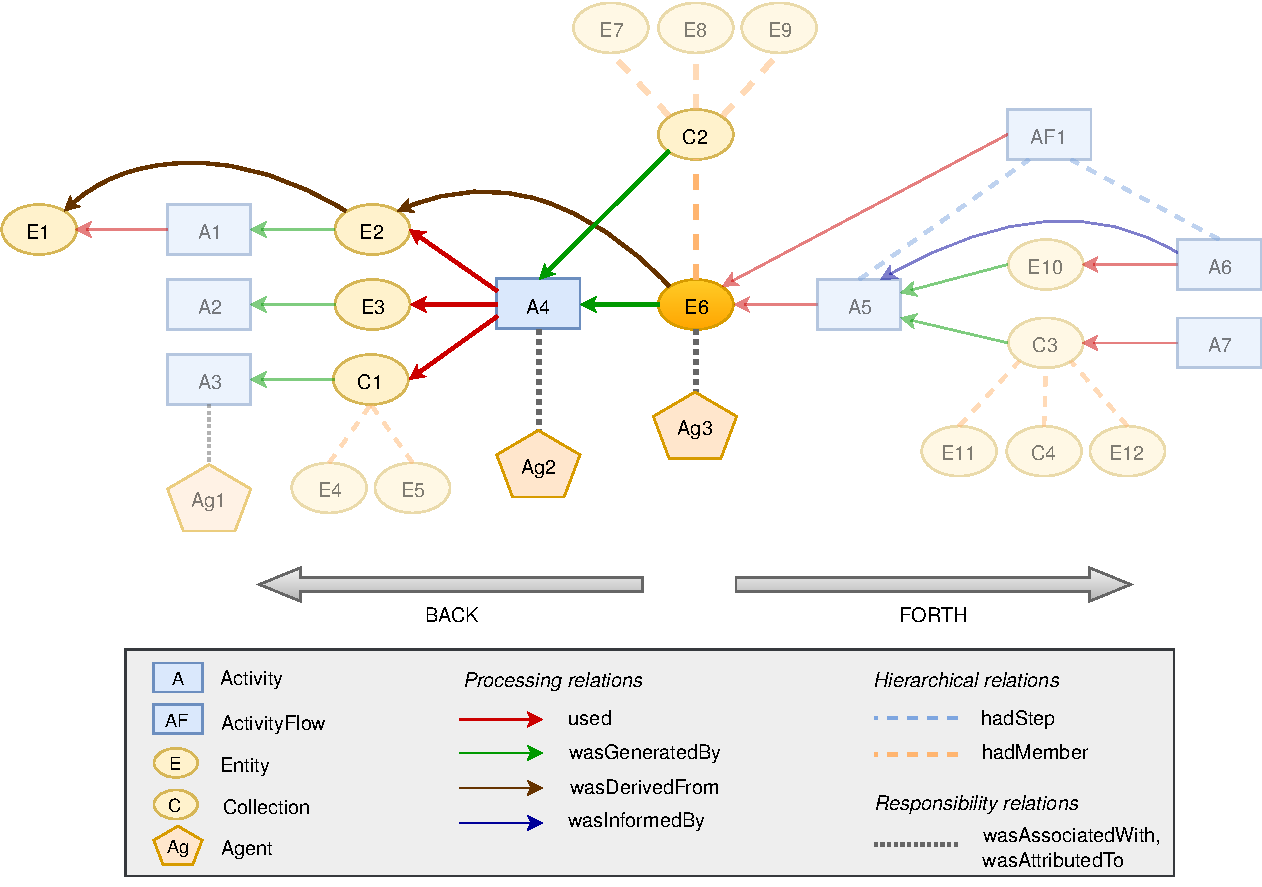
\includegraphics[width=1.0\textwidth]{provenance-graph-example-depth2.pdf}
\caption{An example provenance graph, highlighting the objects and relations returned from a ProvDAL service with \texttt{ID=E6} and \texttt{DEPTH=2}. The BACK and FORTH values for DIRECTION are only important for the processing relations (solid lines). Hierarchial (dashed) and responsibility (dotted) relations are only followed ``upwards'' (to collection/activityFlow) and towards agents by default (unless the optional parameters MEMBERS, STEPS and/or AGENT are set to true.}
\label{fig:provenance-graph-example}
\end{figure}




\paragraph{MEMBERS, STEPS}
The provenance data model defines the hierarchical relations \emph{hadMember} for entity collections and \emph{hadStep} for activityFlows. If a node belongs to a collection or activityFlow, these relations shall be returned as well, independent of the specified tracking direction.
If someone is interested in more details and wants to follow the \emph{members} of an entity collection or the \emph{steps} of an activityFlow, these can be included by setting the optional parameter MEMBERS or STEPS to true, respectively. The default is false. As detailed in DALI \citep{std:DALI}, the values 1 and 0 are equivalent to true and false.

\paragraph{AGENT}
By default, it is recommended to stop any further tracking at an agent node, unless an additional optional parameter AGENT is set to true. Note that this means that the request for any agent will always return just the agent node itself and nothing else, unless AGENT=true is used. An example request if one wants to know which entities and activities an agent has influenced could look like this:\\
\texttt{\{provdal-base-url\}?ID=org:rave\&AGENT=true\&DEPTH=1}.\\
\texttt{DEPTH=1} is used here in order to avoid following the found entities and activities any further (can be omitted, since this is the default for DEPTH).
\newline
%\comment{Maybe it's better to use DEPTH and DIRECTION instead of FORWARD and BACKWARD. Reason: if a service just implements the backward direction, then it's weird to call something ``backward'' if there is no ``forward'' as well. DEPTH is also a commonly used word when refering to graphs and numbers of relations.}



A ProvDAL service MUST implement the parameters ID, DEPTH and FORMAT; the remaining parameters are optional.
If a service does not implement the optional parameters, but they appear in the request, then the service should return with an error.
Please note that according to the DALI specification \citep{std:DALI}, the parameter names are case-insensitive, but the parameter values are not. E.g. \texttt{direcion=FORTH} is allowed, but \texttt{DIRECTION=forth} may not work.

\subsubsection{ProvDAL example use cases}
We provide here a few example use cases for ProvDAL in order to show its usefulness in exploring the provenance
of astronomical datasets, processes or the people and projects involved in producing/performing them.

\begin{itemize}
\item The RAVE DR4 release contains a main table with stellar properties for each observation of a star. Given the RAVE observation ID, retrieve the processing steps
for this specific observation result:

	\begin{verbatim}
	{provdal-base-url}?ID=rave:20121220_0752m38_089&DEPTH=ALL
	\end{verbatim}

The result will not only contain the processing steps (activities), but also entities and agents. The important information can be filtered out by a client application (e.g. use voprov Python package). If a W3C tool shall be used, one needs to transform the response into a W3C compliant serialisation (e.g. for loading the result to ProvStore\footnote{https://provenance.ecs.soton.ac.uk/store/} for further processing).

\item Get the direct progenitor of an entity:
	\begin{verbatim}
	{provdal-base-url}?ID=rave:20121220_0752m38_089&DEPTH=1
	\end{verbatim}
	If this request only returns a collection and not any ``backwards'' information about progenitors, then
	one needs to track the collection further, i.e. repeat the request for the collection entity.

\item Get all datasets that were derived from a specific data file in the CTA pipeline:
	\begin{verbatim}
	{provdal-base-url}?ID=cta:df1&DEPTH=ALL&DIRECTION=FORTH
	\end{verbatim}
	By using \texttt{DIRECTION=FORTH} we can track the dataset and where it was used forward.

\item Find all people that were involved in processing a dataset along with their contact data (if available), so that one can ask them for further information.
	\begin{verbatim}
	{provdal-base-url}?ID=ex:e1&DEPTH=ALL
	\end{verbatim}
 	The ProvDAL request is basically the same as in the first example. From the results the agents need to be filtered.
 	Since the response contains the nodes and relations including all their properties, the contact details for the agents are included as well (if they are stored with the service).

\item Retrieve a VOTABLE serialisation of the provenance for an image from a data collection.
	\begin{verbatim}
	{provdal-base-url}?ID=myproject:img1&DEPTH=ALL&FORMAT=PROV-VOTABLE
	\end{verbatim}
	We use the FORMAT keyword here to retrieve a VOTABLE.
\end{itemize}

ProvDAL is meant to be used to retrieve parts of a provenance graph from a provenance web service. It cannot be used to retrieve information based on specific properties, e.g. the creationTime of an entity or a parameter value for an activity. For such cases, a ProvTAP service can be used (see next section).





\subsubsection{ProvTAP}
ProvTAP is a TAP service implementing the ProvenanceDM data model. The data model mapping is included in the TAP schema. The mapping of ProvenanceDM classes and attributes onto tables and columns of the schema with the appropriate relationships, datatypes, units, utypes and ucds is done similarly to the PROV-VOTABLE serialization. The query response will result in a single table according to the query.
This single table is joining information coming from one or several ``provenance'' tables available in the database.

A special case is considered where ProvenanceDM and ObsCore are both implemented in the same TAP service and queried together. The TAP response is then providing an Obscore table with a ProvenanceDM extension. We can imagine that in the future this could be hard-coded and registered as an ObsProvTAP service.


\TODO{We need more details here! Output of TAP service is NOT a PROV-VOTABLE by default!}

%\TODO{Do we need combined query possibilities, i.e. ask for ObsCore-fields and Provenance fields in one query? Or rather use a 2-step-process, decoupling them from each other?}


%\TODO{Also look at PROV-AQ from the W3C.}

\subsubsection{VOSI availability and capabilities}
\TODO{Still needs to be discussed!}
According to the DALI specification for VO services \citep{std:DALI}, a provenance service implementing ProvDAL and/or ProvTAP must provide a VOSI availability interface as well as a capabilities interface with entries for ProvDAL and/or ProvTAP. The \texttt{standardId}s for these provenance interfaces are:

\begin{verbatim}
ivo://ivoa.net/std/ProvenanceDM#ProvDAL
ivo://ivoa.net/std/ProvenanceDM#ProvTAP
\end{verbatim}

For ProvTAP, the VOSI tables interface also needs to be provided.



\section{Discussion}
\subsection{Links, ids}\label{sec:links_between_data}
It would be convenient, if each data object or even each file 
gets a unique id that can be referenced. The W3C provenance model requires ids
for entities, activities and agents, and they have to be qualified strings, 
i.e. containing a namespace. For example, an activity in the RAVE-pipeline could 
have the id `\texttt{rave:radialvelocity\_pipeline\_20160901}'. Using a namespace for each 
project for these ids will help to make them unique. 

If several copies of a dataset exist, and one of them is corrupted, it would even be useful to know
exactly which copy was used by a given activity. This can be modeled already 
with the existing tools (using a copy-activity), but we doubt that many people
would actually need this level of detail.

IVOIDs and DOI's are potentially good candidates for unique identifiers.


%\subsubsection{Calibration data}
%The calibration dataset consists of images that can be used to calibrate the
%raw data. It is not necessary to mention them explicitly in the model, 
%they are just another dataset that is used by activities with a 
%calibration-method.

%\subsubsection{Quality}
%For expressing the quality of data, we could simply define additional 
%attributes for each \class{Activity}
%or \class{Entity} object, i.e. zero, one, or more properties in the form of
%key-value pairs. We could use a \class{Quality} namespace to mark a keyword
%as quality-related:
%\begin{itemize}
%    \item quality:comment: [some text]
%    \item quality:seeing: [some value]
%\end{itemize}
%The values could range from a float number to free text.


%\subsubsection{Provenance of provenance}
%``Bundles'' are used to name a set of provenance descriptions. It is a type for 
%an entity, and allows to express provenance of provenance. This is probably  
%very interesting for workflow systems.
% -- partially covered already with ActivityFlow

\subsection{Description classes}
This model was established mainly having a database implementation in mind. 
However, it may be better in the long run to store provenance with 
the entities themselves, e.g. as an additional extension in fits-headers.

A model using description classes for defining templates for activities and
entities has an advantage for normalization: the common processes could be 
described once and for all at some place and then be reused when recording
provenance information for certain entities and activities. This \emph{some place} 
is actually the crucial point here.
In an ideal world, ``some place'' could collect all the descriptions from all 
the possible datasets and methods in astronomy, but building such a look-up place 
is a quite challenging task -- it will probably never be complete. There's also 
the issue of persistent identifiers/broken links to consider.
Normalisation is useful for closed systems, e.g. for describing the provenance 
for data produced by a certain pipeline (e.g. MuseWise system) or with 
workflow tools or when a task needs to be repeated many times. However, the VO 
is quite the contrary of a closed system and we need to keep an eye on what is 
actually achievable.

When writing down a simple serialisation of e.g. the provenance for a stacked 
image using the current model including the description classes, it soon becomes quite cumbersome to define 
everything twice: first the descriptions, then the instances. This basically 
doubles the number of entries to describe provenance (unless there is already 
some place with all the descriptions to which we can refer).

Expressing provenance for a stacked image with this smaller set of classes may 
be simpler, but on the other hand constructing a database schema becomes much 
harder. 
We could leave it to the implementors to choose what is more useful for them.
When extracting a serialisation of the provenance information from a provenance 
service, the attributes of the description classes could be combined with 
the corresponding activity/entity classes. This will produce some repetition
(e.g. many entities may have the same descriptive attributes), but 
avoid having too many classes and links between them.
% Note: Harry Enke commented that this sentence is not understandable; 
% we can remove this sentence later on when we have a proper implementation-note section.
%\Note{Descriptions could be present in W3C-conform serialisations, if we 
%put them into entities.}

%\TODO{Check, if PROV-Templates from the W3C (inofficial note) could be used 
%for ActivityDescriptions.}

\subsection{ActivityFlow and implications for multiplicities}
By introducing the \class{ActivityFlow} class, one entity can now have many 
wasGeneratedBy-links to activities. One of them would be the actual generation-activity, 
the other activities can only be activityflows containing this generation-activity.
This is not expressed explicitly in the current model. 

We could introduce an additional abstract class, e.g. \class{AbstractActivity}, with \class{Activity} and 
\class{ActivityFlow} being subclasses to this one. But this adds another layer of complexity 
that we may not want in this data model.

Since we introduced \class{ActivityFlow} mainly for having different view levels, 
we may want to add an attribute \emph{viewLevel} to descriptions of activityflows.

We are planning to test how it all works in implementations, which classes and attributes are 
needed or not and will then adjust the model 
accordingly.

\subsection{VO-DML representation}
We do not yet have a VO-DML compliant representation of the model. This is one 
of the issues to be clarified for the next version.

\subsection{Links to other data models}
Section~\ref{sec:dmlinks} still needs to be expanded further, especially making detailed links with the 
Simulation Data Model will be very useful.


\section{Implementations of the data model for specific use cases}\label{sec:usecases-implementations}
%\subsection{One processing step in PROV-N notation}
%
%\TODO{Put the very simple example here}
%See \url{https://volute.g-vo.org/svn/trunk/projects/dm/provenance/description/prov-example-incl-prototypes.txt}
%and \url{https://volute.g-vo.org/svn/trunk/projects/dm/provenance/description/prov-example-w3c.txt}

\subsection{voprov Python package}



\subsection{Provenance of RAVE database tables (DR4)}
The RAVE survey (Radial Velocity Experiment) recorded spectra for about half a 
million stars. These spectra are processed in a number of steps until the 
derived properties are published in the RAVE data releases at http://www.rave-survey.org.
Providing provenance information for the data, from which spectrum and fibre the
data was coming from and which steps were involved in processing the data, can help scientists
to understand the data and their restrictions and judge their quality.
It would also be useful to be able to compare if, how and why the derived data 
for some stars have changed between different releases.
Provenance information for some major steps of RAVE DR4 was loaded in 
W3C-compatible PROV-N notation and uploaded to the provenance store at 
https://provenance.ecs.soton.ac.uk/store/documents/84064/. This allows to view 
graphs of the workflow by visualising only the main entities, activities and agents 
with their relations. It shows that the provenance concepts explained in this draft 
can be applied directly to data obtained from astronomical observations.

We also tested a Django implementation of the classes in this document along with provenance data stored in an SQLite database. This allows to quickly setup a provenance web service
which gives the possibility to view all instances of a class or details for a single object, 
extract provenance information for single entities (backwards in time) and 
visualise the provenance information. 
More details about this are available in the implementation notes \citep{std:ProvenanceImplementationNote}.




\subsection{Provenance for CTA}

The Cherenkov Telescope Array (CTA) is the next generation ground-based very high energy gamma-ray instrument. It will provide a deep insight into the non-thermal high-energy universe. Contrary to previous Cherenkov experiments, it will serve as an open observatory providing data to a wide astrophysics community, with the requirement to propose self-described data products to users that may be unaware of the Cherenkov astronomy specificities. The proposed structure of the metadata is presented in Figure~\ref{fig:cta_dm}.

\begin{figure}
\centering
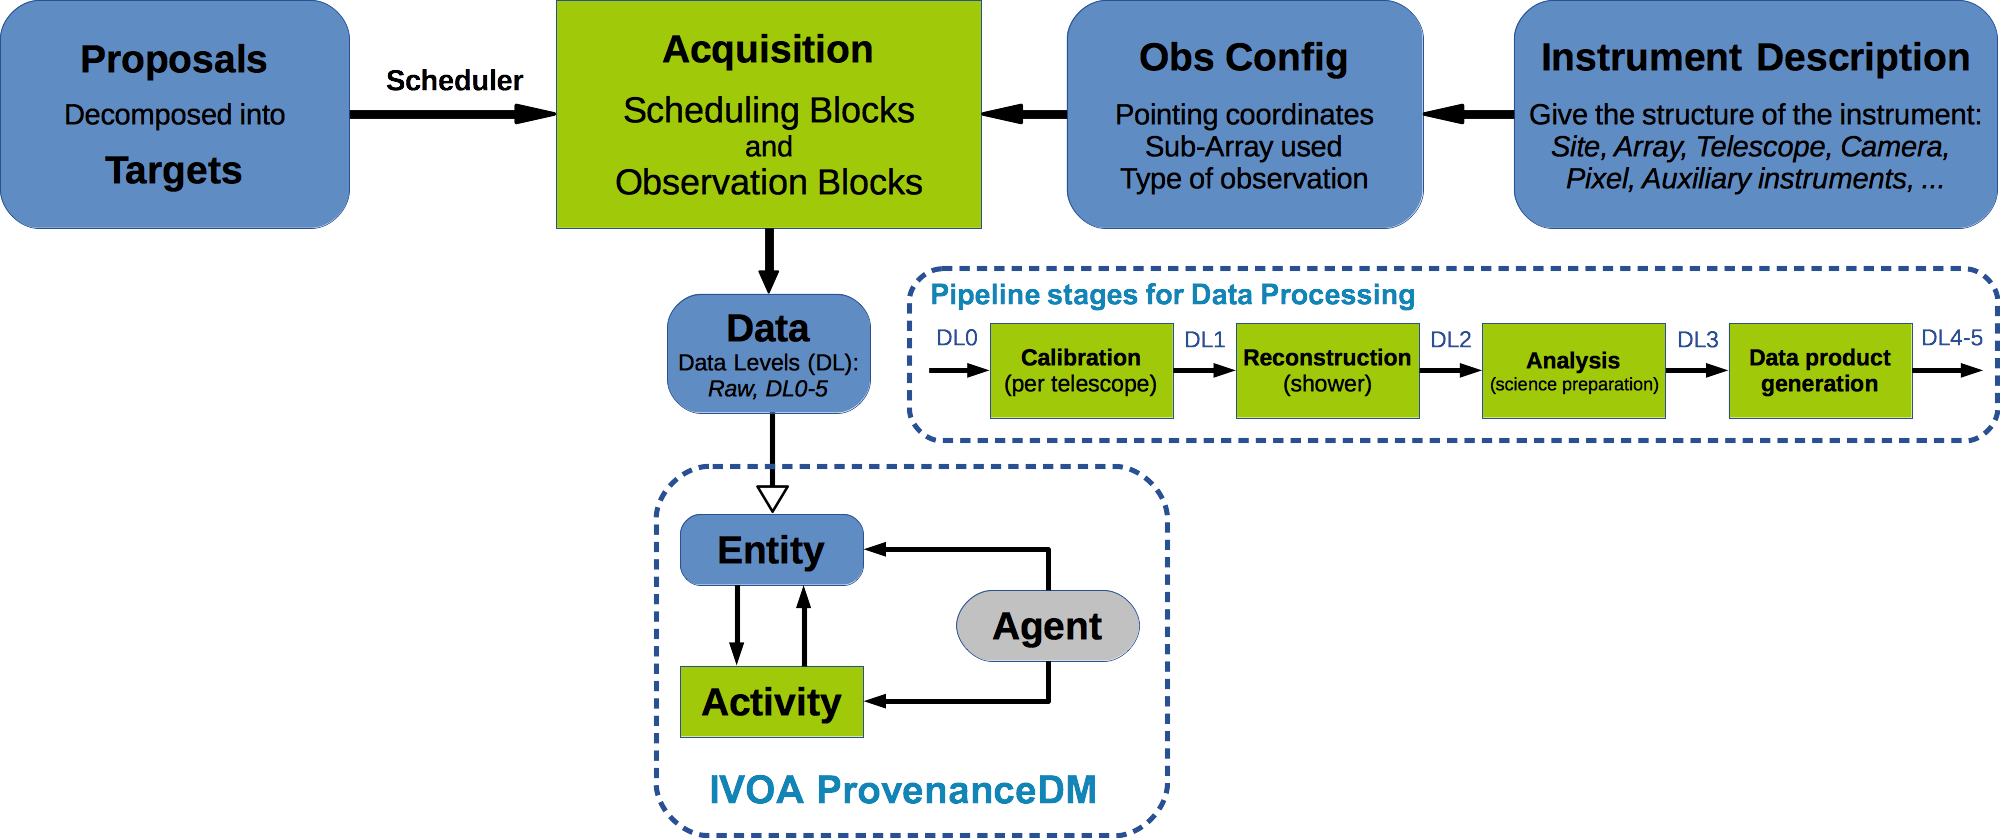
\includegraphics[width=\textwidth]{CTA_DM_high_level.png}
\caption{CTA high level data model structure with Pipeline stages and connection to IVOA ProvenanceDM.}
\label{fig:cta_dm}
\end{figure}

Cherenkov telescopes indirectly detect gamma-rays by observing the flashes of Cherenkov light emitted by particle cascades initiated when the gamma-rays interact with nuclei in the atmosphere. The main difficulty  is that charged cosmic rays also produce such cascades in the atmosphere, which represent an enormous background compared to genuine gamma-ray-induced cascades. Monte Carlo simulations of the shower development and Cherenkov light emission and detection, corresponding to many different observing conditions, are used to model the response of the detectors.  With an array of such detectors the shower is observed  from several points and, working backwards, one can figure out the origin, energy and time of the incident particle. The main stages of the CTA Pipeline are presented inside Figure~\ref{fig:cta_dm}. Because of this complexity in the detection process, provenance information of data products is necessary to the user to perform a correct scientific analysis.

Provenance concepts are relevant for different aspects of CTA :
\begin{itemize}
\item Data diffusion: the diffused data products have to contain all the relevant context information with the assumptions made as well as a description of the methods and algorithms used during the data processing.
\item Pipeline: the CTA Observatory must ensure that data processing is traceable and reproducible.
\item Instrument Configuration: the characteristics of the instrument at a given time have to be available and traceable (hardware changes, measurements of e.g. a reflectivity curve of a mirror, ...)
\end{itemize}

We tested the tracking of Provenance information using the Python prov package inside OPUS\footnote{\url{https://github.com/ParisAstronomicalDataCentre/OPUS}} (Observatoire de Paris UWS System), a job control system developed at PADC (Paris Astronomical Data Centre). This system has been used to run CTA analysis tools and provides a description of the Provenance in the PROV-XML or PROV-JSON serialisations, as well as a graph visualization (see Figure~\ref{fig:cta_prov}).

\begin{figure}
\centering
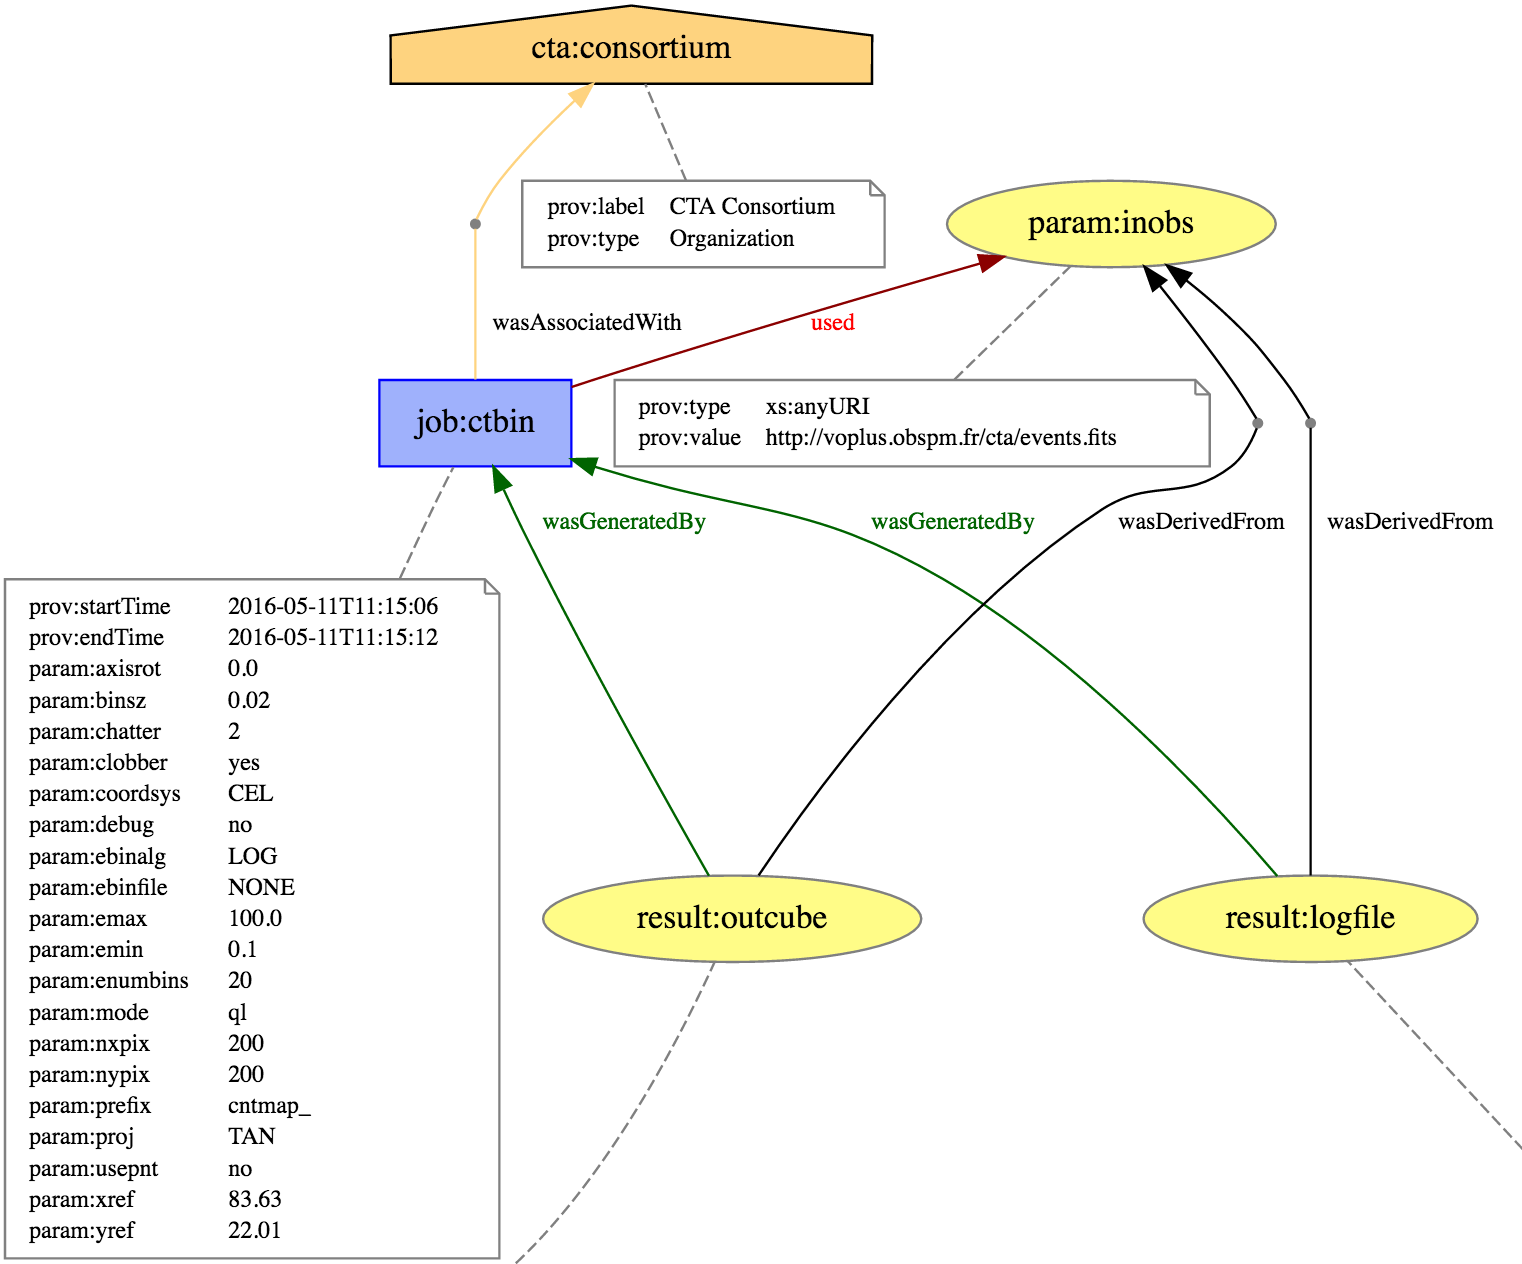
\includegraphics[width=0.8\textwidth]{CTA_prov.png}
\caption{Provenance description of a CTA analysis step.}
\label{fig:cta_prov}
\end{figure}


\subsection{POLLUX database}

POLLUX is a stellar spectra database proposing access to high resolution synthetic spectra computed using the best available models of atmosphere (CMFGEN, ATLAS and MARCS), performant spectral synthesis codes (CMF\_FLUX,SYNSPEC and TURBOSPECTRUM) and atomic linelists from VALD database and specific molecular linelists for cool stars. 

Currently the provenance information is given to the astronomer in the header of the spectra files (depending on the format: FITS, ascii, xml, votables, ...) but in a non normalized description format. 

The implementation of the provenance concepts in a standardized format allows users on one hand to benefit from tools to create, visualize and transform in another format the description of the provenance of these spectra and on a second hand to select data depending on provenance criteria.

\begin{figure}
\centering
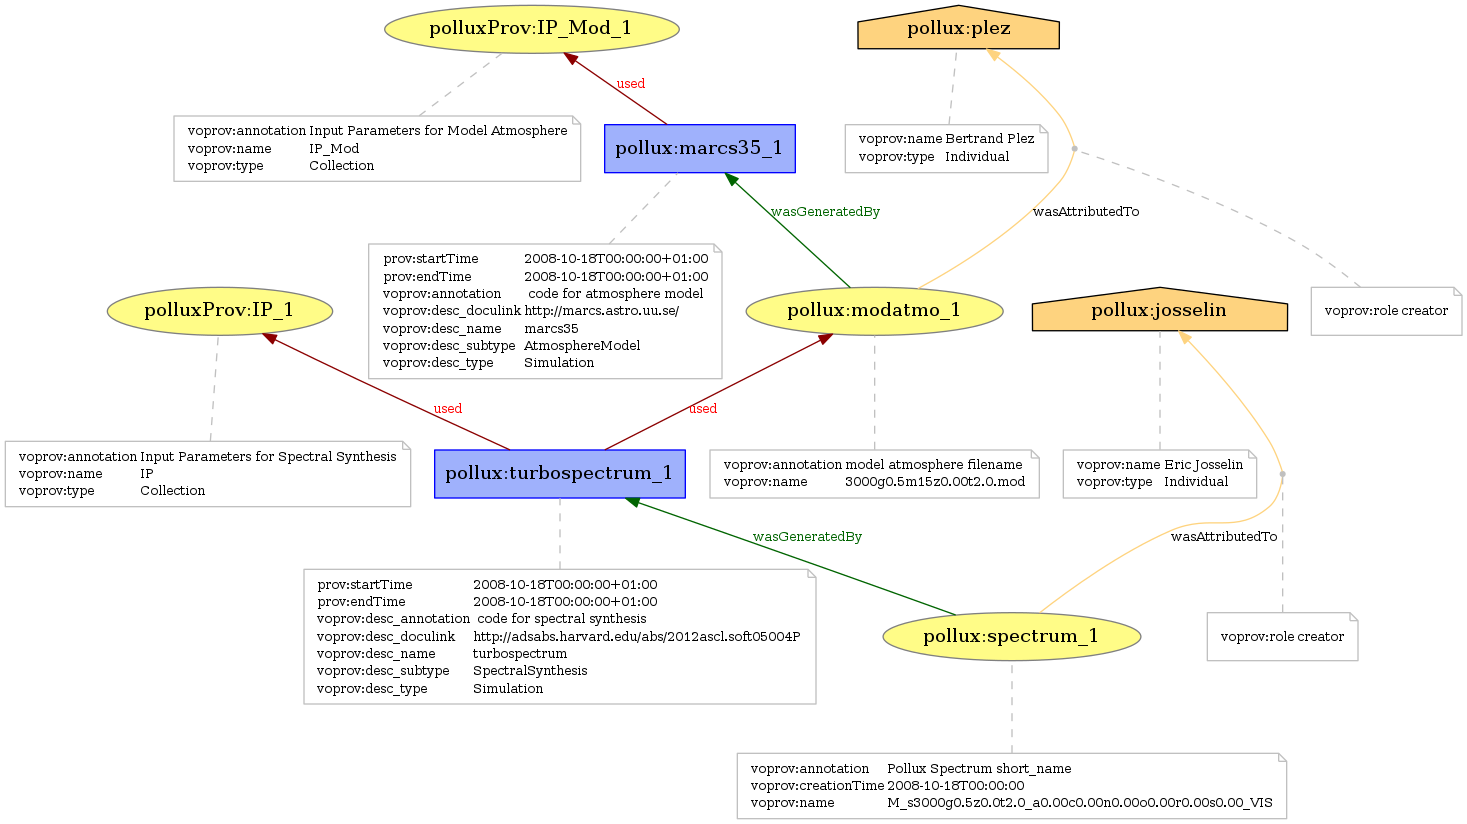
\includegraphics[width=0.9\textwidth]{usecase_Pollux_example1.png}
\caption{Pollux Example 1}
\label{fig:pollux}
\end{figure}

\subsection{HiPS use case}
HiPS is a new all sky organization of pixel data. It is based on HealPix tesselation of the sky on equal area cells (pixels) for a given HealPix order gathered in tiles. Adaptative resolution is achieved by a hierarchy of tiles at increasing order. Sorting and organization is based on a tree of including directories each of those associated with a tile. HiPS specification has entered the IVOA recommendation process and is becoming an interoperability standard.
In the processing chain, HiPS can be seen as a kind of ``legacy level'' for observational data.

An HiPS dataset can be generated either by Aladin in ``hipsgen'' mode or by other softwares.  The processing distinguishes 3 main different methods for estimating cell values: FIRST or NEAREST neighbour, Mean or Median of the neigbouring pixels. Up to 50 parameters can help to tune the processing, among which can be found the higher resolution HealPix order, sky background value to be substracted, border width or mask to apply to original images to avoid including bad area in the computing, etc.

An example of provenance metadata for a HiPS collection generated from a collection of SERC Schmidt plates scanned by CAI (Observatoire de Paris) with the MAMA facility and serialized in PROV-N format is given at 
\url{https://volute.g-vo.org/svn/trunk/projects/dm/provenance/example/HiPS-prov-provn.txt}, the corresponding votable-format is available at \url{https://volute.g-vo.org/svn/trunk/projects/dm/provenance/example/HiPS-prov-vot.xml}.

Here is an extract of the PROV-N serialization:

\begin{verbatim}
Entity
( ivo://CDS/P/MAMA/ESO-R, 
[
prov:label = "ESO-R MAMA HIPS at CDS",
prov:annotation = "This is the HiPS version of ESO Schmidt survey digitized by Mama and processed by CDS",
hips:HiPS_properties = "http://cds.u-strasbg.fr/hips/p/mama/eso-r/properties.txt",
voprov:access_reference = "http://CDS/P/MAMA/ESO-R", // as defined in obscore 
voprov:doculink = "http://cds.u-strasbg.fr/hips/documentation.html#structure",
voprov:dataproduct_type = "voprov:hips_pixels",
voprov:level = 3
]
)

// Relationship
WasAttributedTo(ivo://CDS/P/MAMA/ESO-R, ivo://cds, prov:role = "voprov:creator")

Agent
(ivo://cds,
[
voprov:Name = "CDS",
voprov:contact = "question@astro.unistra.fr",
prov:type = "Organisation"
]
) 

WasGeneratedBy(ivo://CDS/P/MAMA/ESO-R, EHG1, -)

Activity
(EHG1,
[
prov:label = "ESO HiPS generation 1",
prov:startTime = "2016-07-18",
prov:endTime = "2016-07-20",
voprov:annotation = "This activity is final generation of HiPS for ESO Mama survey",
voprov:activityDescription = "HipsgenM"
]
)

ActivityDescription 
(HipsgenM,
[
prov:label = "HiPS Generation MEAN",
prov:type = "HiPSgen",
voprov:subtype = "HiPSgen_MEAN",
voprov:doculink = "http://cds.u-strasbg.fr/HiPSGEN-Documentation"
]
)
\end{verbatim}


\subsection{Lightcurves use case}
TBD. See Provenance webpage in IVOA Twiki for now.



\appendix
\section{Changes from Previous Versions}
% No previous versions yet.
% these would be subsections "Changes from v. WD-..."
% Use itemize environments.
\subsection{Changes from WD-ProvenanceDM-1.0-20161121}
\begin{itemize}
\item More explanations on links to data models in Section~\ref{sec:dmlinks}.
\item Introduced subsections for Section~\ref{sec:dmlinks}, added table with SimDM-links.
\item Renamed \emph{docuLink} to \emph{doculink}
\item Avoid double-meaning of \emph{description} by splitting it up into: 
    \begin{itemize}
    \item \emph{description\_ref}: a foreign key, reference to a description class 
(which could be located at an url as well)
    \item \emph{annotation}: free text description
    \end{itemize}
\item Applied similar naming scheme to \emph{Parameter} and \emph{ParameterDescription}-classes
\item Renamed \emph{Agent.name} to \emph{Agent.label}, so that each class has an id and a label.
\item Renamed Section~\ref{sec:usecases-implementations} to stress that it deals with implementations.
\item Added links to provn and votable-serialization for HiPS-use case, added first part of provn as example in the HiPS-use case section.
\item Corrected attribute names in Table~\ref{tab:datasetmapping}.

\end{itemize}


\section{Implementation details}\label{sec:implementation-details}
In this section we will give more details on the classes and attributes which were used 
in implementations for each use case. This maybe needs to go into a different document, so it can 
be updated without affecting this standard.

TBD.


\bibliography{ivoatex/ivoabib,prov-refs}


\end{document}
